\documentclass{kalliposstd}
\usepackage{caption}
\usepackage{subcaption}
\usepackage{listings}
\lstset{basicstyle=\ttfamily,
  showstringspaces=false,
  commentstyle=\color{red},
  keywordstyle=\color{blue}
}
\usepackage{mathtools}
\usepackage{unicode-math}
\usepackage{multicol}
\def\Lcomm#1{\texttt{\char`\\{}#1}}

%--------------Βιβλιογραφία------------------------------------------------
\usepackage[sorting=none, maxnames=5, style=numeric, bibstyle=numeric]{biblatex}
\DeclareLanguageMapping{english}{greek}
\defbibheading{biboption}{\section*{Βιβλιογραφία}}
\bibliography{chapters/KOY_master}

%-------------------Απλό πλαίσιο με φόντο και τίτλο---------------
\usepackage[framemethod=TikZ]{mdframed}
\mdfdefinestyle{kalboxstyle}{
	skipabove=1.5\topskip,
	skipbelow=.5\topskip,
	rightmargin=0pt,
	leftmargin=0pt,
	%innertopmargin=3pt,
	%innerbottommargin=3pt,
	innerrightmargin=7pt,
	innerleftmargin=7pt,
	topline=false,
	bottomline=false,
	rightline=false,
	leftline=false,
	%linewidth=1pt,
	%roundcorner=0pt,
	%font={},
	%frametitlefont={},
	frametitlerule=true,
	linecolor=black,
	%backgroundcolor=LightBlue,
	fontcolor=black,
	%frametitlebackgroundcolor=LightBlue,
}
\newmdenv[
	style=kalboxstyle,
	backgroundcolor=black!15,
	frametitlebackgroundcolor=black!15
]{kalbox}

%---------Ρυθμίσεις Hyperref / Μεταδεδομένα ----------------------
%-------------------------------------------------------------
%			ΜΕΤΑΔΕΔΟΜΕΝΑ ΚΑΙ ΡΥΘΜΙΣΗ ΕΜΦΑΝΙΣΗΣ ΥΠΕΡΣΥΝΔΕΣΜΩΝ
%-------------------------------------------------------------
\definecolor{linkgray}{gray}{0.2}
\hypersetup{%
%-------------------------------------------------------------
%			ΡΥΘΜΙΣΗ ΕΜΦΑΝΙΣΗΣ ΥΠΕΡΣΥΝΔΕΣΜΩΝ
%-------------------------------------------------------------
    breaklinks=true,
    unicode=true,          	% non-Latin characters in Acrobat’s bookmarks
    pdftoolbar=true,        	% show Acrobat’s toolbar?
    pdfmenubar=true,        	% show Acrobat’s menu?
    pdffitwindow=true,     	% window fit to page when opened
    colorlinks=true,       	% false: boxed links; true: colored links
    linkcolor=linkgray,     	% color of internal links (change box color with linkbordercolor)
    citecolor=linkgray,    	% color of links to bibliography
    filecolor=blue,      	% color of file links
    urlcolor=linkgray,      	% color of external links
%-------------------------------------------------------------
%			ΜΕΤΑΔΕΔΟΜΕΝΑ ΠΟΥ ΣΥΜΠΛΗΡΩΝΟΝΤΑΙ ΑΠΟ ΤΟΝ ΣΥΓΓΡΑΦΕΑ
%-------------------------------------------------------------
    	pdftitle={Οδηγίες για συγγραφείς XeLaTeX},
	pdfsubtitle={Ένας σύντομος Οδηγός},
	pdfauthor={Συγγραφείς με επώνυμο πρώτο γράμμα ονόματος χωρισμένοι με κόμμα},
	pdfsubject={Αντικείμενο του συγγράμματος πχ. υπολογιστικά δίκτυα},
	pdfkeywords={Λέξεις κλειδιά χωρισμένες με κόμμα},
	pdflicenseurl={https://creativecommons.org/licenses/by-nc-sa/4.0/legalcode.el},
% Εναλλακτικά για βιβλία με άδεια cc-non-derivative να χρησιμοποιηθεί
% ο ακόλουθος σύνδεσμος αντί για τον παραπάνω
% https://creativecommons.org/licenses/by-nc-nd/4.0/legalcode.el
%
%-------------------------------------------------------------
%			ΜΕΤΑΔΕΔΟΜΕΝΑ ΠΟΥ ΣΥΜΠΛΗΡΩΝΟΝΤΑΙ ΑΠΟ ΤΗΝ ΚΟΥ
%-------------------------------------------------------------
	pdfcopyright={Copyright © 2021, Κάλλιπος, Ανοικτές Ακαδημαϊκές Εκδόσεις},
	pdfcontactaddress={Εθνικό Μετσόβιο Πολυτεχνείο, Ηρώων Πολυτεχνείου 9, 15780 Ζωγράφου},
	pdfcontactcity={Αθήνα},
	pdfcontactpostcode={15780},
	pdfcontactcountry={Ελλάς},
	pdfcontacturl={https://helpdesk.kallipos.gr/},
	pdfversionid={1},
	pdfpublisher={Κάλλιπος, Ανοικτές Ακαδημαϊκές Εκδόσεις},
	pdfpubtype={book},
	pdflang={el-GR},
	pdfmetalang={el-GR},
	pdfurl={\relax},
	pdfdoi={\relax}
	}%


%-------------------------------------------------------------
%			ΒΙΒΛΙΟ
%-------------------------------------------------------------

\begin{document}
%---------Γραμματοσειρές ----------------------
\setmonofont[Scale=MatchLowercase]{Consolas}
\setmainfont[Mapping=tex-text,Ligatures=Common]{Arno Pro}
\setsansfont[Scale=MatchLowercase,Mapping=tex-text]{Arimo}
\setmathfont[Scale=MatchUppercase]{Asana Math}

%---------Τίτλοι βιβλίου / Μεταδεδομένα ----------------------

\primaryauthor{Κεντρική Ομάδα Υποστήριξης}
\PDFtitle{Οδηγίες για συγγραφείς \XeLaTeX}
\PDFshorttitle{Οδηγίες για συγγραφείς \XeLaTeX}
\PDFdoi{https://www.kallipos.gr/images/kalliposplus/A4/XelatexGuide.pdf}                    %Συμπληρώνεται από την ΚΟΥ (post-production)
\PDFauthor{Κεντρική Ομάδα Υποστήριξης}
\PDFyear{2022}

%------- Εξώφυλλο  ----------------------------------------
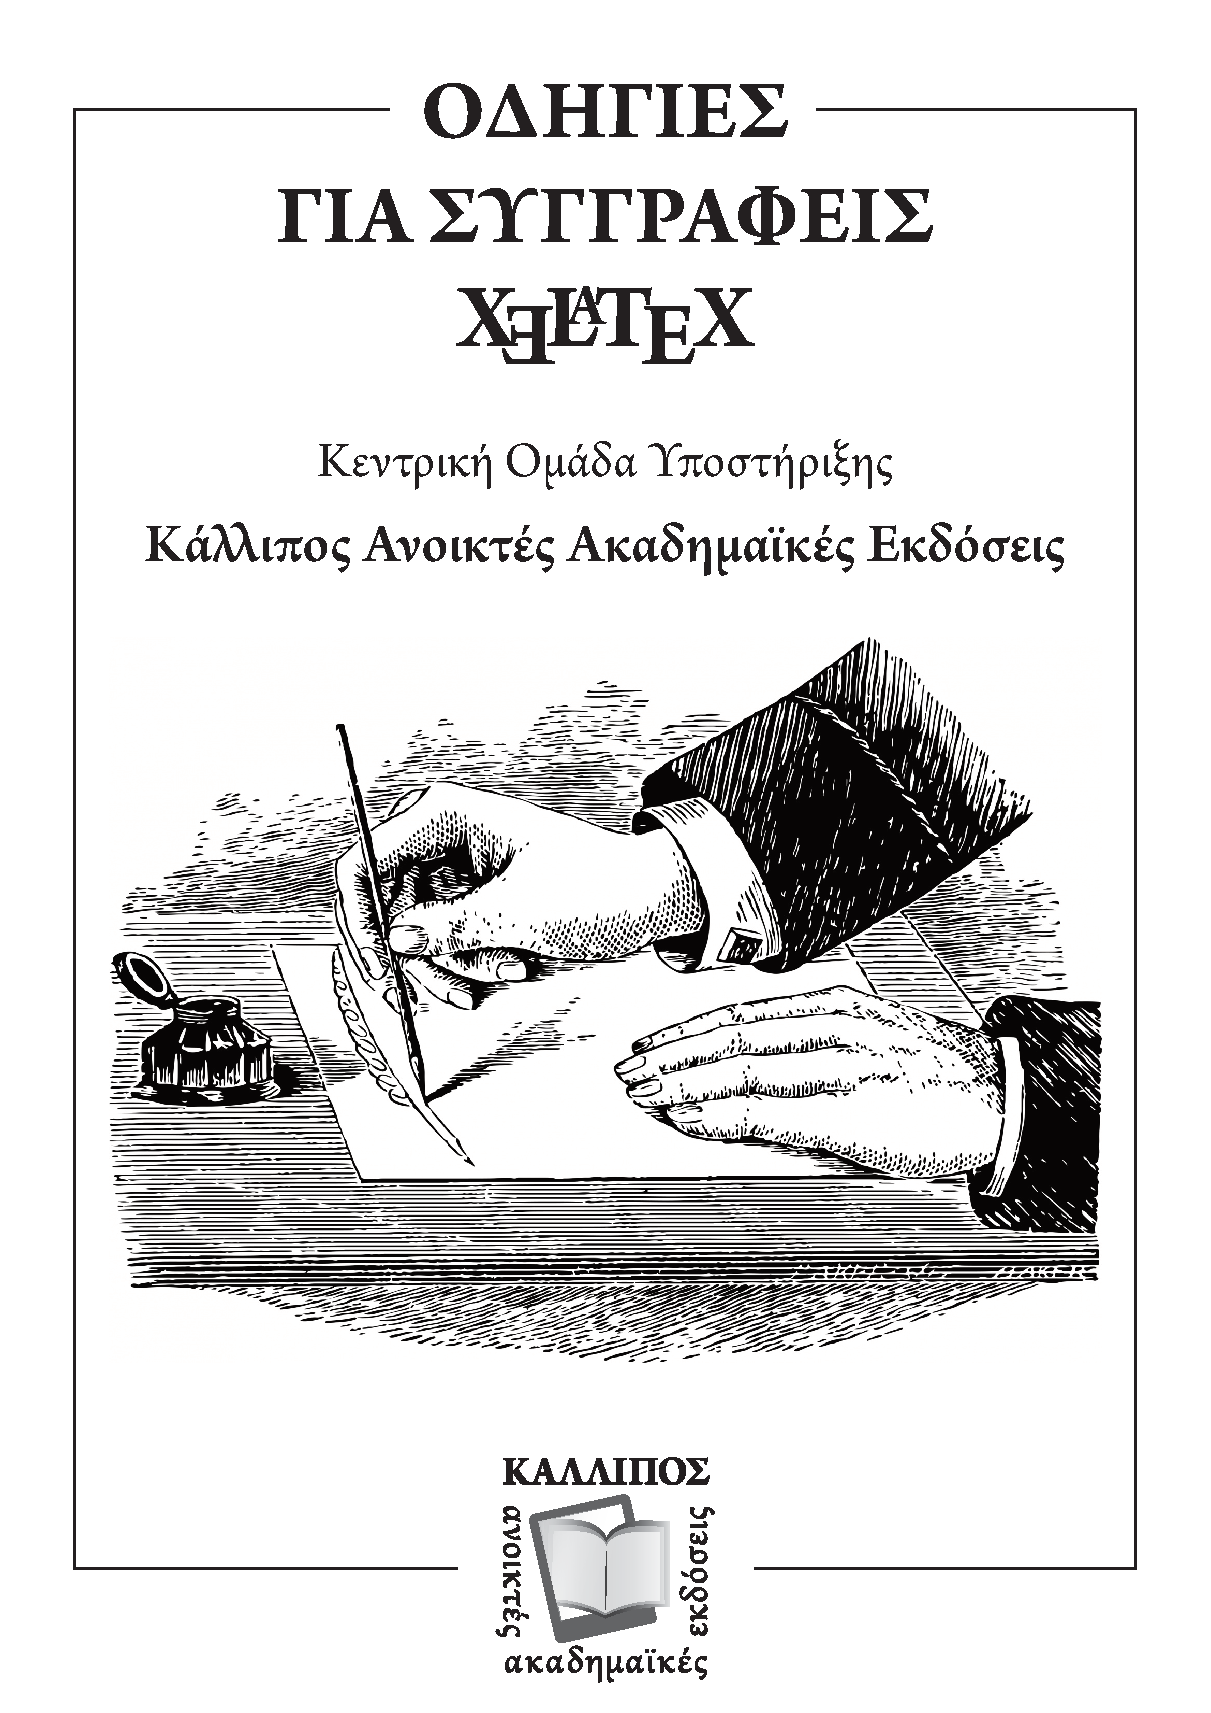
\includepdf[pages=1-2]{images/KOY_cover.pdf}

%------- Στοιχεία αρχικών σελίδων  ----------------------------------------

\soletitlepage{Οδηγίες για συγγραφείς \XeLaTeX}
\begin{authorpage}{Οδηγίες για συγγραφείς \XeLaTeX}[Ένας σύντομος Οδηγός]
\begin{authors}
\textbf{Κεντρική Ομάδα Υποστήριξης}\\ Κάλλιπος, Ανοικτές Ακαδημαϊκές Εκδόσεις\\ Αθήνα \and
\textbf{Όνομα 2ου συγγραφέα}\\ Ιδιότητα\\ Ίδρυμα \and
\textbf{Όνομα 3ου συγγραφέα}\\ Ιδιότητα\\ Ίδρυμα
\end{authors}
\end{authorpage}
\copyrightpage{Σταματίνα Κουτσιλέου}{Αλεξάνδρα Θεοδωράκη}{Γιώργος Παπανικολάου}{978-618-85370-Χ-Χ}
\begin{dedication}
Αφιερώνεται\\
στους συγγραφείς \XeLaTeX,\\
του Έργου ΚΑΛΛΙΠΟΣ+\\
ΚΟΥ
\end{dedication}

%-----------------------------------------------------------------

\frontmatter % ενεργοποπoιεί και το σχετικό pagetstyle
\tableofcontents
\listoffigures
\listoftables
\schapter{Πίνακας συντομεύσεων - ακρωνυμίων} 

\begin{table} [ht] \centering 
\begin{tabular} {p{0.20\linewidth} p{0.80\linewidth}}

\hline
		&	    	\tabularnewline
APA		& American Psychological Association 		\tabularnewline
ΣΕΑΒ		& Σύνδεσμος Ελληνικών Ακαδημαϊκών Βιβλιοθηκών	\tabularnewline
ΚΟΥ		& Κεντρική Ομάδα Υποστήριξης	 		\tabularnewline
ΕΥ		& Επιστημονικά Υπεύθυνος			\tabularnewline
		&	    	\tabularnewline
\hline
\end{tabular}
\label{table:acronyms}
\end{table} 

\schapter{Πρόλογος} % Με την εντολή αυτή δεν έχουμε αρίθμηση αλλά μπαίνει και στον πίνακα περιεχομένων.
\chapterauthor{Κεντρική Ομάδα Υποστήριξης}[Κεντρική Ομάδα Υποστήριξης\\ Κάλλιπος, Ανοικτές Ακαδημαϊκές Εκδόσεις\\ \texttt{https://helpdesk.kallipos.gr}]


        % Αυτή η εντολή χρησιμοποιείται αν έχουμε διαφορετικό συγγραφέα
        % από τον κύριο συγγραφέα του βιβλίου ή δημιουργούμε μια ανθολογία
        % Το δεύτερο optional όρισμα υπάρχει αν θέλουμε να βάλουμε επιπλέον
        % πληροφορίες στον τίτλο του κεφαλαίου αλλά όχι στα περιεχόμενα.

Πρόλογος  θεωρείται το προεισαγωγικό τμήμα του βιβλίου, που τοποθετείται πριν από την εισαγωγή (εφόσον υπάρχει).

Ο πρόλογος είναι ένα πολύ σύντομο κείμενο, συχνά γραμμένο από πρόσωπο διαφορετικό από τον συγγραφέα (από τον εκδότη, από γνωστό ειδικό, από πρόσωπο συνδεόμενο με τον συγγραφέα κ.λπ.). Ο πρόλογος ενίοτε γράφεται και από τον ίδιο τον συγγραφέα, για να περιλάβει σ’ αυτόν γενικότερες πληροφορίες, τεχνικά θέματα του βιβλίου, ευχαριστίες κ.λπ. Εφόσον υπάρχει εισαγωγή, ο πρόλογος προηγείται της εισαγωγής και διαφοροποιείται απ’ αυτήν πλήρως. Εάν δεν υπάρχει εισαγωγή, ο πρόλογος περιέχει στοιχεία που κανονικά θα δίνονταν σε μια εισαγωγή και είναι εκτενέστερος.

\schapter{Εισαγωγή} % Με την εντολή αυτή δεν έχουμε αρίθμηση αλλά μπαίνει και στον πίνακα περιεχομένων.
\chapterauthor{Κεντρική Ομάδα Υποστήριξης}
[Κεντρική Ομάδα Υποστήριξης\\ Κάλλιπος, Ανοικτές Ακαδημαϊκές Εκδόσεις\\ \url{https://helpdesk.kallipos.gr}]  


        % Αυτή η εντολή χρησιμοποιείται αν έχουμε διαφορετικό συγγραφέα
        % από τον κύριο συγγραφέα του βιβλίου ή δημιουργούμε μια ανθολογία
        % Το δεύτερο optional όρισμα υπάρχει αν θέλουμε να βάλουμε επιπλέον
        % πληροφορίες στον τίτλο του κεφαλαίου αλλά όχι στα περιεχόμενα. 

Εισαγωγή είναι το προκαταρκτικό τμήμα βιβλίου, επιστημονικού έργου κ.λπ. 
Η εισαγωγή ενός βιβλίου καταλαμβάνει αρκετές σελίδες και σ’ αυτήν ο συγγραφέας δίνει σημαντικές πληροφορίες για το περιεχόμενο του έργου του, τα κύρια προβλήματα που τον απασχόλησαν, τις γενικές θέσεις του κ.λπ. 


%-------------------------------------------------------------
%			ΚΥΡΙΟ ΜΕΡΟΣ ΤΟΥ ΒΙΒΛΙΟΥ / ΚΕΦΑΛΑΙΑ
%-------------------------------------------------------------

\mainmatter % ενεργοποιεί και το σχετικό pagestyle
\part{Γενικές οδηγίες}
\chapter{Γενικά χαρακτηριστικά και δομή περιεχομένου}\label{chap:character}
\chapterauthor{Κεντρική Ομάδα Υποστήριξης}[Κεντρική Ομάδα Υποστήριξης \\ Κάλλιπος, Ανοικτές Ακαδημαϊκές Εκδόσεις]
\section{Κατηγορίες ηλεκτρονικών βιβλίων }
Στο Έργο ΚΑΛΛΙΠΟΣ+ χρηματοδοτούνται βιβλία/συγγράμματα \footnote{Εφεξής ο όρος θα χρησιμοποιείται εναλλάξ.} τα οποία -από πλευράς
περιεχομένου- ανήκουν σε μία από τις επόμενες κατηγορίες:
\begin{enumerate}
\item \emph{Εγχειρίδια} για Προπτυχιακά \& Μεταπτυχιακά μαθήματα (Νέα συγγράμματα)
\item \emph{Μεταφράσεις} ανοικτών ξενόγλωσσων συγγραμμάτων (open textbooks)
\item \emph{Μονογραφίες} (Νέα συγγράμματα)
\item \emph{Βιβλιογραφικοί Οδηγοί} (Νέα συγγράμματα)
\end{enumerate}

Τα τεχνικά χαρακτηριστικά  που περιγράφονται στις επόμενες παραγράφους αφορούν
κυρίως την ανάπτυξη συγγραμμάτων στις κατηγορίες 1 (Εγχειρίδια) και 3 (Μονογραφίες).
Στις Mεταφράσεις ξενόγλωσσων συγγραμμάτων (textbooks) είναι δυνατόν να ακολουθείται
η δομή και ο μορφότυπος του πρωτότυπου συγγράμματος, ενώ για τους Βιβλιογραφικούς
Οδηγούς, αν και απλούστερο -ως προς τη δομή- είδος συγγραμμάτων, μπορεί να υιοθετείται
o μορφότυπος των κατηγοριών 1 και 3.

\section{Δομή περιεχομένου}
Όπως  καταγράφεται  και  στο  Τεχνικό  Δελτίο  του  Έργου,  στο  πλαίσιο  του  Έργου
ΚΑΛΛΙΠΟΣ+  καλούνται  οι  υποψήφιοι  Συγγραφείς  να  παραδώσουν  συγγράμματα  σε
ηλεκτρονική μορφή με πρωταρχικό  στόχο την αξιοποίησή τους στη διδασκαλία  στα
ελληνικά  Ανώτατα  Εκπαιδευτικά  Ιδρύματα και  στα  Ανώτατα  Στρατιωτικά
Εκπαιδευτικά  Ιδρύματα  της  χώρας  (κυρίως  κατηγορίες  1,  2 και  3  προηγούμενης
παραγράφου). Επομένως, η έκταση του περιεχομένου τους και η διάρθρωσή τους θα πρέπει
να ικανοποιεί τις ανάγκες για τη διεξαγωγή ενός -τουλάχιστον εξαμηνιαίου-  μαθήματος.
Με αφετηρία τα ως άνω, στον Πίνακα \ref{table:megethi} που ακολουθεί παρατίθενται (ως κατάλληλα) τα
\emph{ενδεικτικά} μεσοσταθμικά μεγέθη που θα πρέπει να τηρεί ένα προτεινόμενο ηλεκτρονικό
βιβλίο.

\begin{table} [h] \centering
\caption{Ενδεικτικά μεσοσταθμικά μεγέθη περιεχομένου.}
\vspace{2mm}
\begin{tabular} {l c c}
\hline
	\textbf{Κατηγορία}	&\textbf{Όρια}	&\textbf{Μέσος όρος}\\
\hline
		&	    &	\\
Αριθμός κεφαλαίων	&5 -15 	&10\\
Αριθμός σελίδων	&250 - 350	    &300	\\
Αριθμός σελίδων ανά κεφάλαιο	&25- 35	    &30	\\
	&	    &	\\
\hline
\end{tabular}
\label{table:megethi}
\end{table}

Η γενική δομή ενός εγχειριδίου (προτείνεται να) διαρθρώνεται ως εξής:
\begin{itemize}
\item Ενότητα  1  - Πρώτες  σελίδες  (front pages): Σελίδα  τίτλου,  σελίδα  ISBN  και
Συντελεστών, σελίδα αφιέρωσης (προαιρετική).
\item Ενότητα 2 – Περιεχόμενα (υποχρεωτικό): Πίνακας περιεχομένων.
\item  Ενότητα 3 – Πρόλογος (προαιρετικό): Σημείωμα από τη Συγγραφική Ομάδα ή τρίτα
πρόσωπα.
\item Ενότητα 4 –  Εισαγωγή (προαιρετικό):  Εισαγωγικό σημείωμα από τη Συγγραφική
Ομάδα.
\item  Ενότητα 5 – Κεφάλαια [συμπεριλαμβανομένων, ανά κεφάλαιο, των βιβλιογραφικών
αναφορών (υπο\-χρε\-ω\-τι\-κά) και (προαιρετικά) της θεματικής/επιστημονικής ορολογίας].
\item  Ενότητα 6 – Λίστα σημαντικών μαθησιακών αντικειμένων (προαιρετικό).
\end{itemize}

Όσον αφορά την Ενότητα 5, και ειδικά για την κατηγορία των \emph{Εγχειριδίων για Προπτυχιακά
μαθήματα}, κάθε Κεφάλαιο θα πρέπει να αντιστοιχεί σε μία έως δύο διδακτικές εβδομάδες
ή, αν πρόκειται για Εργαστηριακούς Οδηγούς, να αντιστοιχεί στην εκτέλεση τουλάχιστον
μίας Εργαστηριακής Άσκησης. Επίσης, ένα Κεφάλαιο (και κατά προέκταση το βιβλίο) θα
πρέπει  να  οργανώνεται  στη  μορφή  ενός  ή  περισσοτέρων,  αυτοτελών  στο  μέτρο  του
δυνατού, αντικειμένων  περιεχομένου  (μαθησιακών/εκπαιδευτικών  αντικειμένων).  Οι
παρακάτω κατηγορίες είναι ενδεικτικές, κυρίως σε ό, τι αφορά τα προαιρετικά στοιχεία των
μαθησιακών αντικειμένων:

\begin{table} [h] \centering
\caption{Κατηγορίες περιεχομένου ανά Κεφάλαιο.}
\vspace{2mm}
\begin{tabular} {p{0.55\linewidth} p{0.15\linewidth} p{0.15\linewidth}}
\hline
	\textbf{Πεδίο}	&\textbf{Υποχρεωτικό}	&\textbf{Προαιρετικό}\tabularnewline
\hline
		&	    &	\tabularnewline
Τίτλος		& \centering \centering $\surd$	    &\tabularnewline
Σύνοψη – Περίληψη	&\centering $\surd$	    	&	\tabularnewline
Προαπαιτούμενη γνώση (αναφορές σε άλλα κεφάλαια / βιβλία ή σε λήμματα από καθιερωμένα λεξιλόγια)& \centering $\surd$ &	\tabularnewline
Κυρίως κείμενο	&\centering $\surd$	    &	\tabularnewline
Βιβλιογραφία (Αναφορές/References, και παραπομπές εντός του κειμένου / in-text citations)	&\centering $\surd$	    &	\tabularnewline
Γλωσσάριο/-α επιστημονικών όρων (στην αρχή ή/και στο τέλος του κεφαλαίου) [πχ. πίνακας συντομεύσεων - ακρωνυμίων (στην ελληνική και αγγλική γλώσσα), «ευρετήριο» θεματικών όρων πεδίου]	&	    &\centering $\surd$	\tabularnewline
Προσδοκώμενα μαθησιακά αποτελέσματα/στόχοι	&	    &\centering $\surd$	\tabularnewline
Κριτήρια αξιολόγησης (πχ. φύλλα ερωτήσεων/ασκήσεων αυτοαξιολόγησης/προβλημάτων) με ενδεικτικές απαντήσεις- λύσεις	&	    &\centering $\surd$	\tabularnewline
	&	    &	\tabularnewline
\textbf{Αντικείμενα εντός του κειμένου} &	&		\tabularnewline
\hline
	&	    &	\tabularnewline
Πίνακες	&	    &\centering $\surd$	\tabularnewline
Σχήματα – χάρτες (απλά)	&	    &\centering $\surd$	\tabularnewline
Μαθηματικά αντικείμενα-σύμβολα (σύνολα μαθηματικών ή λογικών σχέσεων)	&	    &\centering $\surd$	\tabularnewline
Αλγοριθμικά αντικείμενα - (ψευδο)κώδικας	&	    &\centering $\surd$	\tabularnewline
	&	    &	\tabularnewline
\hline
\end{tabular}
\label{table:content}
\end{table}

\section{Μεταδεδομένα}
Τα μεταδεδομένα αποτελούν πληροφορία που περιγράφει τα δεδομένα. Ιδιαίτερη βαρύτητα
δίνεται στη συμπλήρωση των μεταδεδομένων (στην ελληνική και στην αγγλική γλώσσα),
τόσο σε επίπεδο βιβλίου όσο και σε επίπεδο Κεφαλαίου, αλλά και στα λοιπά  μαθησιακά
αντικείμενα  που  συγκροτούν Κεφάλαια και βιβλίο. Σε κάθε περίπτωση, η συμπλήρωση
των  μεταδεδομένων  επιτρέπει  την  κατηγοριοποίηση του  παραγόμενου  όγκου
πληροφορίας και διευκολύνει τις αναζητήσεις των χρηστών.

Τα  μεταδεδομένα  θα  συμπληρωθούν  σε  ξεχωριστές  φόρμες  και  θα  παραδοθούν  από  τη
Συγγραφική Ομάδα κατά την υποβολή του τελικού υλικού.

Ειδικότερα, για τα μεταδεδομένα σε επίπεδο βιβλίου ορίζονται στον Πίνακα \ref{table:book_metadata}.

\begin{table} [ht] \centering
\caption{Μεταδεδομένα σε επίπεδο βιβλίου.}
\vspace{2mm}
\begin{tabular} {p{0.55\linewidth} p{0.15\linewidth} p{0.15\linewidth}}
\hline
	\textbf{Πεδίο}	&\textbf{Υποχρεωτικό}	&\textbf{Προαιρετικό}\tabularnewline
\hline
		&	    &	\tabularnewline
Τίτλος		& \centering $\surd$	    &\tabularnewline
Υπότιτλος	&	    	&\centering $\surd$	\tabularnewline
Εναλλακτικός τίτλος &  & \centering $\surd$	\tabularnewline
Συγγραφέας	&\centering $\surd$	    &	\tabularnewline
Συν-συγγραφείς	&\centering $\surd$	    &	\tabularnewline
Υπεύθυνος Κριτικής Ανάγνωσης / Επιμέλειας έκδοσης	&	    &\centering $\surd$	\tabularnewline
Γλωσσικός Επιμελητής	&	    &\centering $\surd$	\tabularnewline
Τεχνικοί Συντελεστές – Γραφιστική επιμέλεια	&	    &\centering $\surd$	\tabularnewline
Θεματική κατηγοριοποίηση (από ελεγχόμενο Κατάλογο
Θεματικών Όρων με τα γνωστικά αντικείμενα / επιστημονικές
εξειδικεύσεις ανά Θεματική Περιοχή / Θεματικό Πεδίο)	&\centering $\surd$	    &	\tabularnewline
Περίληψη	&\centering $\surd$	    &	\tabularnewline
Πίνακας περιεχομένων (σε μορφή κειμένου)	&\centering $\surd$	    &	\tabularnewline
Πληροφορίες σχετικά με τους Συγγραφείς	&\centering $\surd$	    &	\tabularnewline
	&	    &	\tabularnewline
\hline
\end{tabular}
\label{table:book_metadata}
\end{table}


Πέρα από τα γενικά μεταδεδομένα σε επίπεδο βιβλίου, θα πρέπει να καταχωριστούν και
συγκεκριμένα μεταδεδομένα σε επίπεδο Κεφαλαίου. Ειδικότερα, τα μεταδεδομένα σε επίπεδο Κεφαλαίου δίνονται στον πίνακα \ref{table:chapter_metadata}

\begin{table} [h!] \centering
\caption{Μεταδεδομένα σε επίπεδο Κεφαλαίου.}
\vspace{2mm}
\begin{tabular} {p{0.55\linewidth} p{0.15\linewidth} p{0.15\linewidth}}
\hline
	\textbf{Πεδίο}	&\textbf{Υποχρεωτικό}	&\textbf{Προαιρετικό}\tabularnewline
\hline
		&	    &	\tabularnewline
Τίτλος		& \centering $\surd$	    &\tabularnewline
Συγγραφείς	& \centering $\surd$	    	&	\tabularnewline
Βιβλίο, μέρος του οποίου αποτελεί το Κεφάλαιο & \centering $\surd$ & 	\tabularnewline
Θέμα – Θεματικές Περιοχές (από ελεγχόμενο Κατάλογο
Θεματικών Όρων με τα γνωστικά αντικείμενα /
επιστημονικές εξειδικεύσεις ανά Θεματική Περιοχή /
Θεματικό Πεδίο)	&\centering $\surd$	    &	\tabularnewline
Σύνοψη – περίληψη	&\centering $\surd$	    &	\tabularnewline
Πίνακας περιεχομένων (παραγράφων)	&\centering $\surd$	    &	\tabularnewline
Πίνακες μαθησιακών αντικειμένων (πινάκων, σχημάτων, ...)	&	    &\centering $\surd$	\tabularnewline
Προαπαιτούμενη γνώση	&	    &\centering $\surd$	\tabularnewline
Χρονική κάλυψη	&	    & \centering $\surd$	\tabularnewline
Γεωγραφική κάλυψη	&	    &\centering $\surd$	\tabularnewline
	&	    &	\tabularnewline
\hline
\end{tabular}
\label{table:chapter_metadata}
\end{table}

Τέλος, είναι απαραίτητο να συνοδεύονται από μεταδεδομένα τα σημαντικά σε περιεχόμενο
μαθησιακά αντικείμενα (πίνακες, εικόνες, διαδραστικά αντικείμενα κλπ.), τα οποία θα
καταχωρίζονται από τον δημιουργό κατά την υποβολή του συγγράμματος.Τα μεταδεδομένα
ανά κατηγορία περιεχομένου περιγράφονται στις παραγράφους του Κεφαλαίου \ref{chap:writing}
παρακάτω.
\section{Πνευματικά δικαιώματα και χρήση του υλικού}

Ο Συγγραφέας θα παραχωρεί στον ΣΕΑΒ την αποκλειστική Άδεια Εκμετάλλευσης του
έργου του, με την οποία επιτρέπει στον ΣΕΑΒ να ασκήσει ορισμένες από τις εξουσίες του
περιουσιακού δικαιώματος (βλ. Προσάρτημα IV – Όροι και Προϋποθέσεις Συμμετοχής
- Άδεια Εκμετάλλευσης), ωστόσο, αυτοδίκαια, θα διατηρεί το ηθικό δικαίωμα του
δημιουργού.

\chapter{Συγγραφή – Κείμενο – Λοιπά στοιχεία}\label{chap:writing}
\chapterauthor{Κεντρική Ομάδα Υποστήριξης}[Κεντρική Ομάδα Υποστήριξης\\  Κάλλιπος, Ανοικτές Ακαδημαϊκές Εκδόσεις]

\section{Ροή εργασίας}
Το διάγραμμα που ακολουθεί απεικονίζει την προτεινόμενη ροή εργασίας για τη συγγραφή
και τελική παράδοση ενός βιβλίου στο πλαίσιο του Έργου ΚΑΛΛΙΠΟΣ+.

\begin{figure} \centering
\renewcommand{\figurename}{Σχήμα}
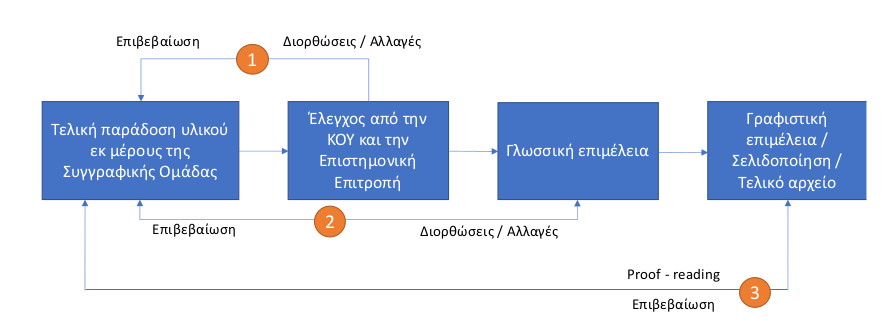
\includegraphics[width=0.8\textwidth]{images/work_flow.png}
\caption[Ροή εργασίας.]{Ροή εργασίας μετά την παράδοση του υλικού εκ μέρους
της Συγγραφικής Ομάδας.}
\label{fig:work_flow}
\end{figure}

Η Συγγραφική Ομάδα οφείλει -στο τέλος του χρονοδιαγράμματος του Έργου- να
παραδώσει το σύνολο του υλικού σύμφωνα με τις προδιαγραφές που καταγράφονται στο
Κεφάλαιο \ref{chap:best-practice}. Στη συνέχεια, η ΚΟΥ και η Επιστημονική Επιτροπή (ΕΕΣΑ) του Έργου (με
τη βοήθεια των Αξιολογητών) θα προβαίνουν στον έλεγχο του υλικού σε επίπεδο τεχνικής
αρτιότητας και επιστημονικής επάρκειας (αντίστοιχα). Τυχόν υποδείξεις για αλλαγές -
διορθώσεις λαθών κλπ. θα αποστέλλονται προς τη Συγγραφική Ομάδα (Βήμα 1). Εφόσον
ολοκληρωθεί με επιτυχία ο έλεγχος του 1ου βήματος, το υλικό θα παραδίδεται σε ειδικό
γλωσσικό επιμελητή. Ο γλωσσικός επιμελητής θα συνεργάζεται στενά με τα μέλη της
Συγγραφικής Ομάδας για διορθώσεις και προσαρμογές (Βήμα 2). Στο τελικό στάδιο, και
αμέσως μετά τη διαδικασία της γλωσσικής επιμέλειας, το υλικό θα παραδίδεται σε ειδικό
ψηφιακό στοιχειοθέτη / γραφίστα για τη σελιδοποίηση και την παραγωγή των τελικών
δοκιμίων του βιβλίου (τόσο σε ηλεκτρονική μορφή όσο και σε τυπογραφικά δοκίμια). Όπως
και στα προηγούμενα στάδια, έτσι και σ’ αυτό το στάδιο ο τελικός έλεγχος θα
πραγματοποιείται από τη Συγγραφική Ομάδα και την ΚΟΥ, από την οποία θα παρέχεται
και η έγκριση για τη δημοσίευση/ανάρτηση του έργου στο Αποθετήριο ΚΑΛΛΙΠΟΣ.
Παρόμοια διαδικασία θα ακολουθείται για την ενδιάμεση παράδοση / παραλαβή υλικού
από τις Συγγραφικές Ομάδες. Ειδικότερα, σε ό, τι αφορά την Ενδιάμεση Αναφορά, η ΚΟΥ
θα προβαίνει σε έλεγχο του συγγραφικού υλικού, σε επίπεδο τεχνικής αρτιότητας, και, σε
συνεργασία με τα μέλη της Επιστημονικής Επιτροπής θα ελέγχει την επιστημονική
επάρκεια, καθώς και το αν τηρούνται οι επιπλέον όροι που τυχόν τέθηκαν κατά το στάδιο
της Αξιολόγησης των Προτάσεων συγγραφής.

Εφόσον οι έλεγχοι του Παραδοτέου υλικού, τόσο κατά την Τελική, όσο και κατά την
Ενδιάμεση Παράδοση/Αναφορά, αξιολογηθούν θετικά, τότε θα αποδεσμεύονται και τα
αντίστοιχα χρηματικά ποσά για την αποζημίωση και των μελών των Συγγραφικών Ομάδων
και των λοιπών Συντελεστών επικουρικών εργασιών.

\section{Δομή – Μορφή κειμένου}
Το κείμενο θα πρέπει να ακολουθεί συγκεκριμένη δομή και μορφή, σύμφωνα με τις
οδηγίες του παρόντος εγγράφου. Η χρήση άλλων εργαλείων
συγγραφής (πχ. LaTeX/XeLaTeX, DocBook) είναι δυνατή μετά από συνεννόηση με την
KOY. Επιπλέον, ο βασικός μορφότυπος για την ανάρτηση και προβολή της ηλεκτρονικής
μορφής του βιβλίου στο Αποθετήριο ΚΑΛΛΙΠΟΣ είναι το PDF.

Εφόσον οι Συγγραφείς έχουν ήδη ολοκληρώσει τη συγγραφή, τότε και μόνο τότε
μπορούν να το παραδώσουν ως έχει, φροντίζοντας απλώς να το συμμορφώσουν, πριν
την παράδοση, στις υποδείξεις που παρέχονται στον παρόντα Οδηγό όσον αφορά την
ονοματοδοσία και δομή των αρχείων (βλ. Κεφάλαιο \ref{chap:best-practice}), τα μεταδεδομένα κλπ.

\subsection{Γενικές οδηγίες διαμόρφωσης και οργάνωσης του κειμένου}
Οι επόμενες οδηγίες θα εφαρμόζονται σε όλα τα πρότυπα αρχεία του κειμένου (πρώτες
σελίδες, περιεχόμενα, εισαγωγή, πρόλογος, κεφάλαια κλπ.):
\begin{itemize}
\item Μορφότυπος (format) αρχείων κειμένου: αρχεία tex
\item Μέγεθος σελίδας: υποχρεωτικά $205\times297$mm. Προαιρετικά για τυπογραφική εκτύπωση $170\times240$mm
\item Περιθώρια: είναι καθορισμένα από το εκάστοτε πρότυπο συγγραφής
\item Διαστήματα: είναι καθορισμένα από το εκάστοτε πρότυπο συγγραφής
\item Γραμματοσειρά (είδος, μέγεθος): arimo (ttf), arno-pro(otf) 11 pt (σε κυρίως κείμενο), 10 pt (σε υποσημειώσεις, λεζάντες).
\item Συλλαβισμός: το κείμενο θα έχει συλλαβισμό
\item Κεφαλίδες, υποσέλιδα: είναι καθορισμένα από το εκάστοτε πρότυπο συγγραφής
\item Σελιδαρίθμηση: είναι καθορισμένη από το εκάστοτε πρότυπο συγγραφής
\item Αρίθμηση-Λεζάντες: Οι λεζάντες των Σχημάτων/Εικόνων κλπ. θα περιέχουν και την
αντίστοιχη αρίθμησή τους. Οι λεζάντες θα γράφονται με τον εξής τρόπο: <Τίτλος λεζάντας
\_αριθμός κεφαλαίου. αριθμός Σχήματος/Εικόνας\_κείμενο λεζάντας>. Οι λεζάντες θα
καταλήγουν σε τελεία (βλ. για παράδειγμα τη λεζάντα στο Σχήμα 2.1 παραπάνω). Τέλος,
συστήνεται να τοποθετούνται κάτω από την Εικόνα, το Σχήμα ή το πολυμεσικό
αντικείμενο και κάτω ή επάνω (προτιμητέο) από τον Πίνακα.
\item Οι μαθηματικοί τύποι και οι χημικές αντιδράσεις μπορούν να γραφούν με την χρήση
των αντίστοιχων πακέτων του \LaTeX / \XeLaTeX\ (Πχ. για χημικές αντιδράσεις chemfig,
mhchem, chemformula κά.).
\item Υπερσύνδεσμοι: Είναι δυνατή η προσθήκη υπερσυνδέσμων (links) σε τοποθεσίες του
διαδικτύου στις οποίες μπορεί να φιλοξενείται περιεχόμενο σχετικό με το σύγγραμμα. Η
ευθύνη διατήρησης του περιεχομένου, ώστε οι υπερσύνδεσμοι να μην παύουν να ισχύουν
(broken links), είναι ευθύνη του Συγγραφέα. Σημειώνεται ότι, αν το URL του συνδέσμου
είναι μεγάλο, δεν είναι απαραίτητο να ενσωματώνεται στο κείμενο, αφού επιτρέπεται να
είναι διαφορετικό το κείμενο του υπερσυνδέσμου από το URL στο οποίο παραπέμπει.
\item Ειδικά σύμβολα: Ιδιαίτερη προσοχή απαιτείται στη χρήση συμβόλων. Για τα ειδικά σύμβολα
που χρησιμοποιούνται στο \LaTeX / \XeLaTeX\ μπορείτε να ανατρέξετε στον υπερσύνδεσμο
\url{https://latex.wikia.org/wiki/List_of_LaTeX_symbols}.
\end{itemize}

\section{Άλλα στοιχεία}

\begin{itemize}
\item Πίνακες: οι Πίνακες δεν πρέπει να έχουν εφέ (effects). Για τη διαμόρφωση των Πινάκων
βλ. παράγραφο \ref{subsec:tables}.
\item Εμφάνιση πολυμεσικών-διαδραστικών αντικειμένων και συνδέσμων (links) εκτός
σύνδεσης δικτύου (offline): Στις περιπτώσεις που δεν είναι δυνατή η σύνδεση σε δίκτυο,
ώστε να είναι ενεργοί οι σύνδεσμοι, απαιτείται περιγραφή του πολυμεσικού/διαδραστικού
αντικειμένου ή του συνδέσμου μέσα στο κείμενο. Γι’ αυτόν τον λόγο, όπου οι συγγραφείς
το κρίνουν απαραίτητο θα γίνεται εισαγωγή (εντός του κειμένου) Πίνακα (με την ακόλουθη
διαμόρφωση) όπου και θα αναφέρονται τα εξής:
\begin{itemize}
\item Τίτλος αντικειμένου/συνδέσμου
\item Τύπος υλικού (πχ. ηχητικό απόσπασμα)
\item Περιγραφή αντικειμένου/συνδέσμου
\end{itemize}
\end{itemize}

\subsection{Περιεχόμενα}

Το βάθος του επιπέδου περιεχομένων δεν πρέπει να ξεπερνά το τέταρτο επίπεδο.

\subsection{Πίνακας Συντομεύσεων-Ακρωνυμίων}

Μετά τα περιεχόμενα θα πρέπει να ακολουθεί Πίνακας (ή Πίνακες) με τις
ελληνόγλωσσες και ξενόγλωσσες συντομεύσεις (ακρωνύμια) που χρησιμοποιούνται στο
κείμενο.

\subsection{Βιβλιογραφία-Αναφορές-Υποσημειώσεις}

Σχετικά με την παρεχόμενη Βιβλιογραφία, ανάλογα με τη συνήθη πρακτική του
επιστημονικού τομέα, οι Συγγραφείς μπορούν να ενσωματώνουν Αναφορές ή
Βιβλιογραφία στο τέλος του κάθε Κεφαλαίου (προτιμητέο, εφόσον κάθε Κεφάλαιο
συνιστά αυτόνομο μαθησιακό αντικείμενο) ή/και συγκεντρωτικά στο τέλος βιβλίου.
Στη Βιβλιογραφία μπορούν να περιλαμβάνονται και αναφορές σε ιστοσελίδες
(δικτυογραφία). Είναι επιθυμητό το να παρέχεται, όπου είναι δυνατό, και το αναγνωριστικό
του αντικειμένου στο οποίο γίνεται αναφορά, για παράδειγμα το DOI για άρθρα σε
περιοδικά, το ISBN για βιβλία κλπ.

Η μορφοποίηση των Αναφορών πρέπει να είναι ομοιόμορφη σε όλο το σύγγραμμα.
Μπορεί να ακολουθεί τη μορφοποίηση της IEEE (χωρίς τις συντομεύσεις απαραίτητα),
προκειμένου για συγγράμματα στις Επιστήμες Μηχανικών κλπ. ή ένα από τα βιβλιογραφικά
συστήματα APA, MLA, Chicago κλπ., προκειμένου για συγγράμματα Ανθρωπιστικών και
Κοινωνικών Επιστημών (πάντως είναι αποδεκτό και οποιαδήποτε άλλο σύστημα,
προφανώς συμβατό με το επιστημονικό πεδίο του συγγράμματος, αρκεί να
εφαρμόζεται με συνέπεια σε όλη την έκταση του κειμένου).
Η προσθήκη υποσημειώσεων (footnotes) στις σελίδες ή στο τέλος του έργου είναι
επιτρεπτή.

\subsection{Πίνακες}\label{subsec:tables}
Ως Πίνακας νοείται πληροφορία δομημένη σε σειρές και στήλες. Αν το αντικείμενο
περιέχει Πίνακα σε εικόνα, τότε αυτό θεωρείται Σχήμα. Η αρίθμηση θα γίνεται με την
εξής διάταξη: <αριθμός Κεφαλαίου.αριθμός Πίνακα> (Πχ. Ο Πίνακας 3.4 θα είναι ο
τέταρτος Πίνακας του Κεφαλαίου 3.). Αυτή η διάταξη αρίθμησης θα αποτελεί μέρος της
λεζάντας η οποία θα βρίσκεται στο κάτω ή το επάνω μέρος του Πίνακα. Χρησιμοποιώντας
αυτήν την αρίθμηση θα γίνεται υποχρεωτικά και αναφορά στον Πίνακα μέσα στο κείμενο
(Πχ. Με βάση τα δεδομένα του Πίνακα 3.4, διαπιστώνεται...).

\subsection{Σχήματα - Εικόνες}\label{sec:images}

Για την επεξεργασία των Εικόνων και των Σχημάτων μπορεί να χρησιμοποιηθεί
οποιοδήποτε σχεδιαστικό πρόγραμμα, πρόγραμμα επεξεργασίας εικόνας, ελεύθερης
πρόσβασης ή εμπορικό. Το τελικό υλικό θα πρέπει να είναι είτε έγχρωμο (colorMode RGB)
είτε ασπρόμαυρο (grayscale), σε κάθε περίπτωση πάντως σε 300 DPI ή περισσότερα. Τα
αποδεκτά πρότυπα είναι τα: SVG, GIF, JPEG, PNG. Όπου δεν είναι δυνατή η χρήση
SVG, προτιμάται η χρήση των JPEG και PNG, καθώς παρουσιάζουν καλύτερες
δυνατότητες απεικόνισης.

Αν είναι δυνατή η επιλογή μεταξύ ψηφιογραφικών (bitmap) (GIF, JPEG, PNG) ή
διανυσματικών (vector) εικόνων, προτιμάται η χρήση των διανυσματικών (SVG)
εικόνων, καθώς προσφέρει τα ακόλουθα πλεονεκτήματα: αφενός ο χρήστης μπορεί να
επιλέξει και να αναζητήσει κείμενο που μπορεί να ενσωματώνεται σ’ αυτές, και αφετέρου
δεν υπάρχει απώλεια στην ποιότητα ανεξάρτητα από την ανάλυση της οθόνης ή τη
μεγέθυνση που επιλέγει ο χρήστης στη συσκευή ανάγνωσης.

Επίσης, στην περίπτωση των ψηφιογραφικών εικόνων προτιμάται η αποθήκευση σε
πρότυπο που δεν μειώνει την ποιότητα της εικόνας (όπως το PNG), έναντι προτύπων που,
προκειμένου να συμπιέσουν την εικόνα, επιφέρουν μείωση της ποιότητας (όπως το JPG).
Για τη συμπίεση των εικόνων είναι προτιμότερο να χρησιμοποιούνται υπηρεσίες τύπου
TinyPNG, οι οποίες μειώνουν αισθητά το μέγεθος αποθήκευσης χωρίς ορατή απώλεια
πληροφορίας.

Το Πρωτογενές Υλικό για τη δημιουργία Σχημάτων και Εικόνων (για παράδειγμα,
αρχεία Visio, Adobe Photoshop, Adobe Illustrator ή οποιοδήποτε αρχείο στον μορφότυπο
του αντίστοιχου λογισμικού στο οποίο έγινε η επεξεργασία της Εικόνας) θα πρέπει να
συμπεριλαμβάνεται στον φάκελο “images” (βλ. Κεφάλαιο \ref{chap:best-practice}).

Τέλος, η αρίθμηση θα γίνεται με την εξής διάταξη: <αριθμός Κεφαλαίου.αριθμός
Σχήματος> (Πχ. Το Σχήμα 3.6 θα είναι το έκτο Σχήμα του Κεφαλαίου 3.). Η παραπάνω
διάταξη αρίθμησης θα αποτελεί μέρος της λεζάντας η οποία θα βρίσκεται στο κάτω μέρος
του Σχήματος. Χρησιμοποιώντας την ως άνω αρίθμηση θα γίνεται υποχρεωτικά και
αναφορά στο Σχήμα μέσα στο κείμενο (Πχ. Στο Σχήμα 3.6 απεικονίζεται...).

\subsection{Μαθηματικά αντικείμενα - εξισώσεις}

Επιτρέπεται, η εισαγωγή εξισώσεων απευθείας μέσα στο κείμενο. Όσον αφορά εκείνες στις οποίες χρειάζεται να
γίνει αναφορά, θα πρέπει να εισάγονται με το περιβάλλον \texttt{equation} ώστε να αριθμούνται σειριακά
μέσα στο Κεφάλαιο στη μορφή (αριθμός Κεφαλαίου.αριθμός Εξίσωσης), Πχ.
\begin{equation}
\label{eq:11_19}
F_{ST}=\frac{H_{T}-\bar{H}_{S}}{H_{T}}
\end{equation}
\subsection{Αλγόριθμοι}

Οι αλγόριθμοι και τα τμήματα κώδικα μπορούν να εισάγονται ως αυτόνομα μαθησιακά
αντικείμενα. Συγκεκριμένα, ένας αλγόριθμος μπορεί να παρέχεται είτε σε κάποια από τις
διαδεδομένες γλώσσες προγραμματισμού (πχ. Java, C) είτε σε μορφή ψευδοκώδικα.

\section{Πολυμεσικό υλικό και διαδραστικά αντικείμενα}

Στην κατηγορία αυτή περιλαμβάνεται το πολυμεσικό υλικό (video, ήχος κλπ.), καθώς και
τα αντικείμενα τα οποία εμφανίζουν κινούμενο και διαδραστικό περιεχόμενο, όπως, για
παράδειγμα, παρουσιάσεις, κουίζ, εκπαιδευτικά παιχνίδια, animations, χάρτες κλπ. Οι
συγκεκριμένες κατηγορίες υλικού είναι προαιρετικές, επομένως η ανάπτυξη, η
συμπερίληψή τους στη δομή του βιβλίου και η παράδοσή τους θα πραγματοποιείται μετά
από συνεννόηση με την ΚΟΥ.

Τα πολυμεσικά αντικείμενα θα τοποθετούνται στους φακέλους “video” και “audio”, ενώ τα
διαδραστικά στον φάκελο “interactive” (βλ. Κεφάλαιο \ref{chap:best-practice}). Αν για τα διαδραστικά
αντικείμενα απαιτείται η λειτουργία ξεχωριστών υπολογιστικών ή απεικονιστικών δομών
(πχ. websites), \emph{η Συγγραφική Ομάδα είναι υπεύθυνη για τη διασφάλιση της συνεχούς
λειτουργίας των εν λόγω δομών}.

\subsection{Ήχος}
Τα ηχητικά αποσπάσματα (audioclips) που περιλαμβάνονται στο υλικό του βιβλίου θα
κωδικοποιούνται σε μορφότυπο MP3 ή σε MP4 με κωδικοποίηση AAC. Επίσης, θα
πρέπει να συμπεριλαμβάνονται στο Πρωτογενές Υλικό, και, ειδικότερα, να αποθηκεύονται
στον φάκελο “audio” (σε ξεχωριστά αρχεία και συνοδευόμενα από τα μεταδεδομένα τους,
βλ. Κεφάλαιο \ref{chap:best-practice}).

\subsection{Βίντεο}

Χρειάζεται προσοχή στην ενσωμάτωση των βίντεο, καθώς δεν είναι εξασφαλισμένη η
αναπαραγωγή τους. Ειδικά σε παλαιότερους ηλεκτρονικούς αναγνώστες, τα βίντεο δεν θα
αναπαράγονται λόγω χαμηλού ρυθμού ανανέωσης (refresh rate) της οθόνης και (λόγω)
υπολογιστικής ισχύος. Βέβαια, εφόσον τα βίντεο είναι σε πρότυπο MPEG-4 (MP4) με
κωδικοποίηση H.264, αφενός υποστηρίζονται, αφετέρου είναι δυνατή η αναπαραγωγή
τους σε νεότερες συσκευές και tablets.

\section{Μαθησιακά αντικείμενα – Μεταδεδομένα}\label{par:metadata}

Τα μαθησιακά αντικείμενα αποτελούν αυτόνομες και επαναχρησιμοποιήσιμες μονάδες
ψηφιακού υλικού που μπορούν να αξιοποιηθούν για τη διδασκαλία και τη μάθηση. Εφόσον
οι Συγγραφείς επιλέξουν να ορίσουν μέρος του περιεχομένου του έργου τους ως μαθησιακό
αντικείμενο (πχ. πίνακας, εικόνα, εξίσωση, κώδικας, απόσπασμα βίντεο ή ήχου, διαδραστικό
αντικείμενο κλπ.), οφείλουν να το καταχωρίσουν στον αντίστοιχο φάκελο (βλ. Κεφάλαιο
4), συμπληρώνοντας παράλληλα και τα απαραίτητα μεταδεδομένα, όπως αυτά
αποτυπώνονται στον Πίνακα \ref{table:learning_object_metadata}.

\begin{table} [ht] \centering
\caption{Μεταδεδομένα μαθησιακών αντικειμένων}
\vspace{2mm}
\begin{tabular} {p{0.55\linewidth} p{0.15\linewidth} p{0.15\linewidth}}
\hline
	\textbf{Πεδίο}	&\textbf{Υποχρεωτικό}	&\textbf{Προαιρετικό}\tabularnewline
\hline
		&	    &	\tabularnewline
Τίτλος		& \centering $\surd$	    &\tabularnewline
Περιγραφή	& \centering $\surd$	    	&	\tabularnewline
Δημιουργοί 	&  	& \centering $\surd$	\tabularnewline
Λέξεις-κλειδιά	&\centering $\surd$	    &	\tabularnewline
Θεματική Κατηγορία (από ελεγχόμενα λεξιλόγια) &\centering $\surd$	    &	\tabularnewline
	&	    &	\tabularnewline
\hline
\end{tabular}
\label{table:learning_object_metadata}
\end{table}

\section{Αποδεκτοί και επιθυμητοί μορφότυποι παραδοτέων κειμένων}
\begin{itemize}
\item Ενδιάμεσοι (αποδεκτοί) μορφότυποι για το κείμενο: αρχεία tex
\item Τελικοί μορφότυποι: pdf (υποχρεωτικά)
\end{itemize}

\chapter{Καλές πρακτικές συγγραφής - Παράδοση υλικού}\label{chap:best-practice}
\chapterauthor{Κεντρική Ομάδα Υποστήριξης\\  Κάλλιπος, Ανοικτές Ακαδημαϊκές Εκδόσεις}

\section{Καλές πρακτικές συγγραφής}
\subsection{Γενικές οδηγίες}
Εφόσον κάθε Συγγραφέας έχει το δικό του προσωπικό ύφος γραφής, οι παρακάτω οδηγίες
περιορίζονται απλώς στην επισήμανση καλών πρακτικών που θα ήταν χρήσιμο να
ληφθούν υπόψη κατά τη διάρκεια της συγγραφής, δεδομένων και των ιδιαιτεροτήτων ενός
ηλεκτρονικού βιβλίου:
\begin{itemize}
\item Η ηλεκτρονική μορφή του βιβλίου δίνει τη δυνατότητα (άμεσης) μεταφοράς στο
σημείο στο οποίο κάποιος θέλει να παραπέμψει μέσα στο κείμενό του, οπότε η
παρουσίαση του υλικού μπορεί να γίνει χωρίς την (περιττή) επανάληψη
πληροφοριών.
\item Κατά τη μεταφορά υλικού από άλλη πηγή, όταν γίνεται αντιγραφή και
επικόλληση, θα πρέπει να δίνεται προσοχή για να μην
μεταφέρονται στο κείμενο εντολές στοιχειοθέτησης που μπορεί να χαλάσουν την
ήδη υφιστάμενη. Επίσης, συστήνεται να ελέγχεται η ορθογραφία του, καθώς είναι
συχνό φαινόμενο να μεταφέρονται λάθη, όπως και χαρακτήρες που δημιουργούν
πρόβλημα.
\end{itemize}
Γενικότερα, να αποφεύγεται η γραφή με αποκλειστική χρήση κεφαλαίων (κυρίως στις
επικεφαλίδες και στους τίτλους/υπότιτλους), καθώς κάτι τέτοιο δυσχεραίνει την
ανάγνωση, ενώ ορισμένες φορές δημιουργεί και αμφισημία.
\subsection{Καλές πρακτικές συγγραφής \XeLaTeX}
Κατά τη συγγραφή σε \XeLaTeX\ είναι καλό να μην γράφουμε μεγάλες γραμμές κώδικα γιατί στη
συνέχεια δυσχεραίνεται η αποσφαλμάτωσή του. Αρκετοί επεξεργαστές διαθέτουν λειτουργικότητα
που βοηθά τη συγγραφή. Συνήθως 80-100 χαρακτήρες ανά γραμμή είναι αρκετοί.

Κατά τη συγγραφή σημαντικό είναι να εισάγουμε κατατοπιστικά σχόλια ώστε να μπορούμε
με ευκολότερο τρόπο να ανατρέξουμε στις περιοχές του κώδικα που επιθυμούμε.

Προσπαθούμε πάντα να διατηρήσουμε των αριθμό των πακέτων που φορτώνονται στα απολύτως
απαραίτητα για τη σωστή λειτουργικότητα του κειμένου μας.

\section{Υλικό προς παράδοση}\label{package}

Στο Πρωτογενές Υλικό της συγγραφικής δραστηριότητας περιλαμβάνονται: αρχεία
κειμένου, εικόνες, σχήματα, βίντεο, διαδραστικά αντικείμενα, αριθμητικά δεδομένα
παραγωγής σχημάτων (datasets) κλπ.

Αναλυτικά, το Πρωτογενές Υλικό θα παραδίδεται σε ξεχωριστούς φακέλους ως εξής:
\begin{itemize}
\item \textbf{Φάκελος “01\_text”}: Εδώ εντάσσεται το συνολικό αρχείο ή/και τα αρχεία του
κειμένου (για τις περιπτώσεις ξεχωριστών αρχείων ανά Κεφάλαιο). Το όνομα του
κάθε αρχείου θα δίνεται ως εξής: <Ε\-πώ\-νυ\-μο Κύριου Συγγραφέα>\_master (για τις
περιπτώσεις ενός αρχείου, πχ. Papadopoulos\_master.docx) ή <Επώ\-νυ\-μο Κύριου
Συγγραφέα>\_chapter\_n (Papadopoulos\_chapter\_01.docx), όπου n θα είναι ο
αντίστοιχος αριθμός του κάθε Κεφαλαίου. Ο συνηθισμένος αποδεκτός μορφότυπος
κειμένου είναι το docx. Δεν αφορά τους συγγραφείς \LaTeX.
\item \textbf{Φάκελος “02\_tex”}: Ο εν λόγω φάκελος αφορά αποκλειστικά Συγγραφείς που
συγγράφουν σε \LaTeX, \XeLaTeX. Τα αρχεία .tex θα πρέπει να είναι οργανωμένα ως
εξής: ένα κύριο αρχείο .tex με όνομα <Ε\-πώ\-νυ\-μο Κύριου Συγγραφέα>\_master.tex
το οποίο θα περιλαμβάνει αναφορές σε ξεχωριστά αρχεία .tex, ένα για κάθε
Κεφάλαιο. Στον υποφάκελο "chapters" θα πρέπει να συμπεριλαμβάνονται τα
ξεχωριστά αρχεία .tex για κάθε Κεφάλαιο με ονομασία <Επώνυμο Κύριου
Συγγραφέα>\_chapter\_n (Papadopoulos\_chapter\_01.tex). Στον υποφάκελο "images" τα επεξεργασμένα τελικά αρχεία εικόνων που ενσωματώνονται στα αρχεία .tex. Σε κάθε περίπτωση, το
σύνολο των αρχείων θα πρέπει να επιτρέπει τη μετατροπή των αρχείων .tex στο
πλήρες PDF του συγγράμματος. Στον φάκελο .tex συμπεριλαμβάνεται
υποφάκελος PDF, όπου τοποθετούνται, τόσο το PDF του συγγράμματος, όσο και
αρχεία PDF για κάθε Κεφάλαιο ή Παράρτημα, ξεχωριστά. Η ονοματοδοσία των
αρχείων PDF θα πρέπει να ακολουθεί τους ίδιους κανόνες με την ονοματολογία των
αρχείων .tex. Οι συγγραφείς μπορούν απλώς να αντιγράψουν στον φάκελο “02\_tex” το περιεχόμενο του φακέλου που συγγράφουν εφόσον ακολουθούν το πρότυπο του Έργου.
\item \textbf{Φάκελος “03\_tables”}: Εδώ εντάσσονται οι Πίνακες σε μορφή Εικόνας εφόσον
αποτελούν μαθησιακό αντικείμενο, συμπεριλαμβανομένων και των μεταδεδομένων
(βλ. παράγραφο \ref{par:metadata}). Με εξαίρεση τυχόν μεταδεδομένα οι συγγραφείς \LaTeX, \XeLaTeX\ δεν χρειάζεται να συμπεριλάβουν Πίνακες σε αυτόν τον φάκελο, εκτός εάν έχουν ενσωματώσει στο βιβλίο τους Πίνακες με τη μορφή pdf (βλέπε σχετικά σελ. \pageref{subsub:tables}).
\item \textbf{Φάκελος “04\_images”}: Εδώ εντάσσονται τα Πρωτογενή (raw) αρχεία
Εικόνων/Σχημάτων κλπ. (για παράδειγμα, αρχεία Visio, Adobe Photoshop, Adobe
Illustrator ή οποιοδήποτε αρχείο στον μορφότυπο του αντίστοιχου λογισμικού στο
οποίο έγινε η επεξεργασία της Εικόνας) και τα αρχεία των Εικόνων/Σχημάτων όπως
αυτά εισάγονται στα προγράμματα επεξεργασίας κειμένου (MS Word ή \LaTeX)
(βλ. παράγραφο \ref{sec:images}). Τα Πρωτογενή αρχεία θα αποθηκεύονται στον υποφάκελο
raw\_images, ενώ τα παραγόμενα αρχεία που χρησιμοποιούνται για την εισαγωγή
τους στο κείμενο θα τοποθετούνται στον υποφάκελο final\_images. Τα περιεχόμενα του final\_images
ουσιαστικά είναι τα ίδια με τον υποφάκελο "images" του φάκελου "02\_tex" για τους συγγραφείς
\LaTeX, \XeLaTeX~. Σε κάθε περίπτωση η ονοματοδοσία όλων των αρχείων θα πρέπει να ακολουθεί τις
οδηγίες της παραγράφου \ref{package}.
\item \textbf{Φάκελος “05\_math”}: Δεν αφορά τους συγγραφείς \LaTeX, \XeLaTeX\,
\item \textbf{Φάκελος “06\_audio”}: Εδώ εντάσσονται τα αρχεία ήχου,
\item \textbf{Φάκελος “07\_video”}: Εδώ εντάσσονται τα αρχεία video,
\item \textbf{Φάκελος “08\_interactive”}: Εδώ εντάσσονται τα διαδραστικά αντικείμενα.
\end{itemize}

Όπου είναι απαραίτητο θα πρέπει να συμπεριλαμβάνεται και το αρχείο των μεταδεδομένων
ανά μαθησιακό αντικείμενο.

Σε κάθε περίπτωση, όταν για την προβολή ή και αναπαραγωγή του κάθε στοιχείου
(μαθησιακού αντικειμένου) χρειάζονται περισσότερα του ενός αρχεία (πχ. βιβλιοθήκες
javascript, αρχεία CSS), τότε όλα τα αρχεία θα δίνονται σε ένα συμπιεσμένο αρχείο (zip).
Η ΚΟΥ του Έργου μπορεί να αναλάβει τη μετατροπή σε ηλεκτρονική μορφή PDF, εφόσον
το Πρωτογενές Υλικό έχει μορφοποιηθεί όπως περιγράφεται στον παρόντα Οδηγό.
Όσον αφορά ειδικές περιπτώσεις, επιβάλλεται το να προηγείται συνεννόηση με την ΚΟΥ
για τον τρόπο και τη μορφή παράδοσης του τελικού υλικού.

Το σύνολο του υλικού θα τοποθετείται σε έναν φάκελο, το όνομα του
οποίου θα σχηματίζεται από το επώνυμο του κύριου Συγγραφέα και τις πρώτες λέξεις του
τίτλου, έως και τέσσερις λέξεις:\\
EPONYMO\_KYRIOU\_SYGRAFEA\_TITLOS\_SYGRAMATOS.zip.

Ο εν λόγω φάκελος θα συμπιέζεται σε ένα αρχείο zip (με το ίδιο όνομα με τον φάκελο), το οποίο και θα υποβληθεί ηλεκτρονικά. Για τη διευκόλυνσή σας μπορείτε να καταφορτώσετε συμπιεσμένο αρχείο με τη δομή των φακέλων που περιγράφεται παραπάνω από τον σύνδεσμο \href{https://www.kallipos.gr/images/kalliposplus/A4/EPONYMO_KYRIOU_SYGRAFEA_TITLOS_SYGRAMATOS.zip} {<<φάκελοι πρωτογενούς υλικού>>}.

\chapter{Γλωσσικός Οδηγός προς Συγγραφείς - Συγγραφικές Ομάδες}\label{chap:lang-guide}
\chapterauthor{Κεντρική Ομάδα Υποστήριξης\\  Κάλλιπος, Ανοικτές Ακαδημαϊκές Εκδόσεις}

\section{Γενικές οδηγίες}
Κατά τη χρήση αντωνυμιών, βεβαιωθείτε ότι είναι σαφές σε ποιον όρο γίνεται η
αναφορά. Προτιμήστε τη χρήση αντωνυμιών στα διάφορα γένη (ο οποίος, η οποία, το
οποίο), αριθμούς (οι οποίοι, οι οποίες, τα οποία) και πτώσεις, αντί του αναφορικού που,
καθώς η έκφραση των νοημάτων και η συσχέτιση με τον όρο αναφοράς γίνεται με
μεγαλύτερη ακρίβεια.
\subsection{Ορολογία στην ελληνική γλώσσα ή/και σε άλλες γλώσσες}
Η χρήση των όρων πρέπει να γίνεται με βάση τα ακόλουθα:
\begin{itemize}
\item Κατά την πρώτη αναφορά ακρωνυμίου ή αρκτικόλεξου, γράψτε τον όρο αναλυμένο,
ακολουθούμενο μέσα σε παρένθεση από το ακρωνύμιο ή αρκτικόλεξό του:
Πχ. Ο Σύνδεσμος Ελληνικών Ακαδημαϊκών Βιβλιοθηκών (ΣΕΑΒ) συγκαλεί τα μέλη
του σε Γενική Συνέλευση δύο φορές τον χρόνο.
Είτε χρησιμοποιείτε τελείες στο ακρωνύμιο/αρκτικόλεξο είτε όχι (συστήνεται!),
τηρήστε με συνέπεια την επιλογή σας σε όλη την έκταση του κειμένου.
Σε προτάσεις που τελειώνουν με αρκτικόλεξα/ακρωνύμια για τα οποία χρησιμοποιείτε
τελεία, μην την επαναλαμβάνετε για να δηλώσετε ότι ολοκληρώνεται η περίοδος του λόγου:
Πχ. Ο συντονισμός των εκδηλώσεων γίνεται από τον Σ.Ε.Α.Β.
\item Κατά την πρώτη αναφορά ελληνικού όρου του οποίου μεταφραστικό ισοδύναμο υπάρχει
σε άλλη γλώσ\-σα, οι δύο όροι θα πρέπει να εμφανίζονται μαζί (με τον ξενόγλωσσο όρο
να ακολουθεί μέσα σε παρένθεση). Πχ. Η πολυτροπική επισημείωση (multimodal annotation) δίνει τη δυνατότητα
επισημείωσης σε υλικό που περιέχει εικόνα, βίντεο, ήχο, είτε συνδυασμούς των
προαναφερθέντων μέσων.

Σε περίπτωση που ξενικός όρος αντιστοιχεί σε περισσότερους του ενός ελληνικούς όρους
(ή το αντίστροφο), τηρήστε με συνέπεια την επιλογή που θα κάνετε. Πχ., ο όρος name
identities αποδίδεται ως ονοματικές οντότητες, ονόματα οντοτήτων κλπ. Η επιλογή σας θα
πρέπει να είναι μία και να μην εμφανίζονται πολλαπλές αποδόσεις που μπορεί να
δημιουργήσουν σύγχυση.
\item Σε περίπτωση που η ίδια έννοια εκφράζεται με όρους που ο ένας επικαλύπτει ή έχει
αντικαταστήσει τον άλλον, δηλώστε ποιος είναι ο όρος που χρησιμοποιείται στην
τρέχουσα επιστημονική ορολογία, κάνοντας, όμως, αναφορά και σ’ αυτούς που
χρησιμοποιούνταν στο παρελθόν. Για παράδειγμα: Σακχαρώδης Διαβήτης τύπου 1 /
Diabetes mellitus type 1 (γνωστός και ως διαβήτης τύπου 1 / type 1 diabetes, ο οποίος μέχρι
πρότινος αναφερόταν ως ινσουλινοεξαρτώμενος διαβήτης / insulin dependent diabetes ή
νεανικός διαβήτης / juvenile diabetes).
\item Τέλος, παραθέστε, μετά τα περιεχόμενα, στην αρχή του συγγράμματος, έναν Πίνακα με
όλα τα αρκτικόλεξα/ακρωνύμια που χρησιμοποιήσατε (στην ελληνική και στην αγγλική
γλώσσα), αναλυμένα (ολογράφως). Εναλλακτικά, συντάξτε έναν Πίνακα όπου θα
αναφέρονται αντιστοιχισμένοι οι ελληνικοί όροι με τους όρους στις άλλες γλώσσες και
ενσωματώστε τον στο Ευρετήριο (index) ή παραθέστε τον μετά, στο τέλος του
συγγράμματος.
\end{itemize}
\subsection{Κύρια Ονόματα}
Είναι προτιμότερο να διατηρείτε τα ανθρωπωνύμια και τοπωνύμια στη γλώσσα
προέλευσής τους (πχ. Steve Jobs, Stéphane Mallarmé), με εξαίρεση τις περιπτώσεις για τις
οποίες υπάρχει καθιερωμένη γραφή στην ελληνική γλώσσα (πχ. Λονδίνο, Σαίξπηρ κλπ.).
Σε περίπτωση που χρειαστεί (ή αποφασίσετε) να τα μεταγράψετε, ακολουθήστε τις οδηγίες
που δίνονται στο \emph{Διοργανικό Εγχειρίδιο Σύνταξης Κειμένων}
(\url{https://publications.europa.eu/code/el/el-4100500el.htm}).

Κατά την αναφορά σε χώρες και νομίσματα (κυρίως στις συντομογραφίες τους),
εφαρμόστε ό,τι προτείνει το \emph{Διοργανικό Εγχειρίδιο Σύνταξης Κειμένων}
(\url{http://publications.europa.eu/code/el/el-
370100.htm,http://publications.europa.eu/code/el/el-370303.htm#code})
ή υιοθετήστε κάποιο από τα ισχύοντα ISO (πχ. 639-2).

\subsection{Λίστες και απαρίθμηση}
Κατά τη χρήση λίστας, υιοθετήστε την ακόλουθη λογική:
\begin{itemize}
\item Σε απαρίθμηση ονομάτων ή φράσεων, ξεκινήστε με άνω και κάτω τελεία, γράψτε το
πρώτο γράμμα μικρό, χωρίστε με κόμμα και βάλτε τελεία μετά το τελευταίο στοιχείο:
\begin{itemize}
\item ένα,
\item δύο,
\item τρία.
\end{itemize}

{ή}

\begin{itemize}
\item πρώτο στοιχείο,
\item δεύτερο στοιχείο,
\item τρίτο στοιχείο.
\end{itemize}
\item Σε απαρίθμηση ολοκληρωμένων προτάσεων, ξεκινήστε κάθε πρόταση με κεφαλαίο
και στο τέλος της βάλτε τελεία.
\begin{itemize}
\item Εδώ αρχίζει η λίστα.
\item Εδώ συνεχίζεται η λίστα.
\item Εδώ ολοκληρώνεται η λίστα.
\end{itemize}
\end{itemize}
\textbf{Σημείωση:} Για Καλές Πρακτικές Συγγραφής, συστήνεται, προς αξιοποίηση, ο «Οδηγός
Γλωσσικής Επιμέλειας» της Δράσης ΚΑΛΛΙΠΟΣ (β’έκδοση \footnote{Γενικά, μεταβαίνοντας στη διεύθυνση \url{https://publications.europa.eu/code/el/el-4100000.htm} (Τελευταία ενημέρωση: 28.2.2019) δηλ. σε οδηγίες για την παρουσίαση των κειμένων στην ελληνική γλώσσα, αποκτάτε πρόσβαση στις αντίστοιχες ενότητες του Διοργανικού εγχειρίδιου, κάποιες από τις οποίες ενδέχεται -σε ορισμένα σημεία- να έχουν επικαιροποιηθεί σε σχέση με τα αναγραφόμενα στον ως άνω Οδηγό της Δράσης. Όσον αφορά δύο (2) υπερσυνδέσμους του Οδηγού, οι οποίοι στη β’ έκδοσή του δεν «ανοίγουν», παρατίθενται εδώ επικαιροποιημένοι, για ενδεχόμενη χρήση τους
[\url{http://ebooks.edu.gr/ebooks/v/html/8547/2009/Grammatiki\_E-ST-Dimotikou\_html-apli/},
\url{https://eeyem.eap.gr/wp-content/uploads/2016/09/APA\_ver2.pdf} (αφορά την 6η έκδοση APA), ενώ
σημειώνεται πως πρόσφατα η APA έχει εκδώσει και 7η έκδοση, ενδεικτικά
βλ. \url{https://apastyle.apa.org/style-grammar-guidelines/references/examples}].} ,
\url{http://repository.seab.gr/bitstream/1/27/5/20150728\_Glossikis\_Epimeleias\_v2.pdf}), όπου
παρέχονται αναλυτικές Οδηγίες/Υποδείξεις για ζητήματα γλώσσας/περιεχομένου που θα
αντιμετωπίσουν και θα κληθούν να επιλύσουν τα μέλη των Συγγραφικών Ομάδων, καθώς
και οι Συντελεστές επικουρικών εργασιών.

\chapter{Αδειοδότηση εικόνων \& ήχου – Πνευματικά δικαιώματα }\label{chap:ip-rights}
\chapterauthor{Κεντρική Ομάδα Υποστήριξης\\  Κάλλιπος, Ανοικτές Ακαδημαϊκές Εκδόσεις}

\section{Αδειοδότηση εικόνων \& ήχου – Πνευματικά δικαιώματα}

Σχετικά με την αδειοδότηση για τη συμπερίληψη εικόνων και ήχου, στον παρακάτω
σύνδεσμο έχει αναρτηθεί Υπόδειγμα για αίτημα προς παραχώρηση άδειας χρήσης υλικού,
καθώς και Δήλωση παραχώρησης από τον Δικαιούχο (στα ελληνικά).

Κατεβάστε το Υπόδειγμα Αίτησης (\href{https://www.kallipos.gr/images/kalliposplus/A4/Ypodeigma\_Epistoli\_gia\_lipsi\_adeias\_xrisis\_ylikou.docx}{$\downarrow$}).

\part{Συγγραφή με \XeLaTeX}
\chapter{Συγγραφή με την κλάση kalliposstd }\label{chap:kallipos-std}
\begin{refsection}
\chapterauthor{Α. Συρόπουλος}
\chapterauthor{Γ. Παπανικολάου}
\begin{summary}{Σε αυτό το κεφάλαιο:}
Περιγράφονται οι εντολές και τα ειδικά περιβάλλοντα του τύπου εγγράφου βιβλίο kalliposstd. Δίνονται επίσης παραδείγματα χρήσης τους. \\
\textbf{Προαπαιτούμενη γνώση}:~Βασικές γνώσεις συγγραφής σε περιβάλλον~\XeLaTeX.
\end{summary}
\section{Λίγα λόγια για τον τύπο εγγράφου βιβλίο Kallipos standard}
Ο τύπος εγγράφου <<βιβλίο Kallipos standard>> (kalliposstd) δημιουργήθηκε από τον Α. Συρόπουλο με σκοπό να διευκολύνει τους συγγραφείς \XeLaTeX\ του Έργου ΚΑΛΛΙΠΟΣ+. Παρέχει τη δυνατότητα μορφοποίησης των βιβλίων με σχετικά ενιαίο τρόπο και απαλλάσσει τους συγγραφείς από την ανάγκη να δαπανήσουν επιπρόσθετο χρόνο ασχολούμενοι με τη μορφοποίηση του βιβλίου τους.

Ο τύπος εγγράφου kalliposstd είναι μια προέκταση του τυποποιημένου τύπου εγγράφου book που παρέχει κάθε διανομή \TeX~. Εισάγει έναν περιορισμένο αριθμό από ειδικά περιβάλλοντα και εντολές ώστε να διευκολυνθούν οι συγγραφείς \XeLaTeX\ κατά τη διαδικασία της συγγραφής.

\section{Προετοιμασία για συγγραφή}

\subsection{Εργασία στον τοπικό υπολογιστή}
Οι συγγραφείς \XeLaTeX\ συνήθως χρησιμοποιούν τα εργαλεία συγγραφής με τα οποία είναι εξοικειωμένοι. Αν
είστε νέος στο \XeLaTeX\ μπορείτε να δοκιμάσετε γνωστά εργαλεία συγγραφής, όπως τα προγράμματα TexMaker, TexWorks, ή απλώς κάποιο πρόγραμμα επεξεργασίας κειμένου όπως emacs, vim, gedit, notepad++ και πολλά άλλα. Αν είστε νέος στο \XeLaTeX\ μπορείτε εύκολα και απλά να ξεκινήσετε τη συγγραφή τροποποιώντας το αρχείο KOY\_master.tex και τα αρχεία του φακέλου \textbf{chapters}.

Στο μέλλον ο τύπος εγγράφου kalliposstd θα διατεθεί και σε online πλατφόρμες όπως οι ShareLatex και Overleaf.

\subsection{Καταφόρτωση του πρότυπου}
Μπορείτε να καταφορτώσετε τον kalliposstd με τη μορφή συμπιεσμένου αρχείου από τον ακόλουθο υπερσύνδεσμο:

\url{https://www.kallipos.gr/images/kalliposplus/A4/kalliposstd.zip}

Για να αποσυμπιέσετε το αρχείο χρησιμοποιήστε το γραφικό περιβάλλον (Windows και GNU/LINUX).

\subsubsection{Περιεχόμενα του αρχείου kalliposstd.zip}
Στον φάκελο \textbf{fonts} περιέχονται οι γραμματοσειρές που συνοδεύουν τον kalliposstd. Προκειμένου να μπορέσετε να εργαστείτε με τον kalliposstd θα χρειαστεί πρώτα να εγκαταστήσετε τις γραμματοσειρές όπως περιγράφεται παρακάτω.

Στον φάκελο \textbf{chapters} περιέχονται τα κεφάλαια του Οδηγού για τους συγγραφείς \XeLaTeX\, ενώ το βασικό αρχείο (master file) του οδηγού βρίσκεται στον αρχικό φάκελο (KOY\_master.tex).

Στον φάκελο \textbf{images} τοποθετούνται τα αρχεία εικόνων που χρησιμοποιείτε στο βιβλίο σας.

Στον φάκελο \textbf{pdf} περιέχεται ο οδηγός σε μορφή pdf. Στον φάκελο pdf τοποθετείτε τα αρχεία pdf που παράγετε, τόσο το πλήρες βιβλίο, όσο και τα επιμέρους κεφάλαια και παραρτήματα σε ξεχωριστά αρχεία pdf.

Σημειώνεται ότι η δομή του φακέλου διευκολύνει τη διαδικασία παράδοσης του υλικού, καθώς το μόνο που χρειάζεται να κάνουν οι συγγραφείς  \XeLaTeX\ είναι να αντιγράψουν τα περιεχόμενα του φακέλου στον φάκελο \textbf{02\_tex} (βλέπε σελ. \pageref{package}).

Tο αρχείο \textbf{kalliposstd.cls} ορίζει τον τύπο εγγράφου kalliposstd. Στην
προκαθορισμένη λειτουργία του τύπου εγγράφου Kalliposstd θεωρείται ότι χρησιμοποιούμε τον τύπο
εγγράφου \texttt{book} με τις επιλογές \texttt{twoside} και \texttt{12pt}.

O χρήστης του αρχείου \texttt{kalliposstd.cls}, θα πρέπει να χρησιμοποιεί τη μηχανή \XeLaTeX.
Έτσι, η πρώτη γραμμή του αρχείου του θα έχει την παρακατω μορφή:
\begin{center}
\verb=\documentclass{kalliposstd}=
\end{center}
ή
\begin{center}
\verb=\documentclass[draft]{kalliposstd}=
\end{center}

\subsection{Εγκατάσταση γραμματοσειρών}
\subsubsection{Λειτουργικό σύστημα GNU/LINUX - Συστήματα τύπου UNIX }

Οι γραμματοσειρές διαμοιράζονται μαζί με το πρότυπο στα συμπιεσμένα αρχεία arno-pro.zip και arimo.zip. Για να εγκατασταθούν αποσυμπιέστε τα αρχεία από το γραφικό περιβάλλον ή με τη βοήθεια της εντολής:
\begin{verbatim}
unzip arno-pro.zip
\end{verbatim}
Στη συνέχεια μπορείτε να εγκαταστήσετε τις γραμματοσειρές με έναν από τους παρακάτω τρεις τρόπους:
\begin{enumerate}
\item Αντιγράψτε τον αποσυμπιεσμένο φάκελο Arno Pro (αρχεία otf) στον φάκελο /usr/share/fonts/opentype και τον φάκελο arimo στον φάκελο /usr/share/fonts/truetype. Απαραίτητο είναι να διαθέτετε δικαιώματα διαχειριστή:
\begin{verbatim}
sudo cp -R $HOME/path_to_folder/arno-pro /usr/share/fonts/opentype/
sudo cp -R $HOME/path_to_folder/arimo /usr/share/fonts/truetype/
\end{verbatim}
αντικαθιστώντας το \verb=/home/username/path_to_folder/= με το μονοπάτι για τον αποσυμπιεσμένο φάκελο. Αφού πραγματοποιήσετε την αντιγραφή των αρχείων εκτελέστε την εντολή:
\begin{verbatim} sudo fc-cache -f -v
\end{verbatim}
\item Εναλλακτικά, μπορείτε να εγκαταστήσετε τις γραμματοσειρές για το περιβάλλον του χρήστη σας αντιγράφοντάς τες στον φάκελο /home/.fonts. Αν ο φάκελος δεν υπάρχει, μπορούμε να τον δημιουργήσουμε.
\item Τέλος, με διπλό κλικ πάνω στα αρχεία των γραμματοσειρών ανοίγει η εφαρμογή \emph{Font Viewer} που μας επιτρέπει την εγκατάστασή τους από το γραφικό περιβάλλον.
\end{enumerate}
Για την αναπαραγωγή του παρόντος Οδηγού θα χρειαστεί να εγκαταστήσετε με τον ίδιο τρόπο τη γραμματοσειρά Consolas που μπορείτε να καταφορτώσετε από τη διεύθυνση \url{https://www.freefonts.io/downloads/consolas/}
\subsubsection{Λειτουργικό σύστημα WINDOWS 10}
Για εγκατάσταση των γραμματοσειρών στο λειτουργικό σύστημα WINDOWS 10:
\begin{enumerate}
\item Ανοίξτε το control panel και στη συνέχεια ακολουθήστε τη διαδρομή \textbf{Control Panel} > \textbf{Appearance and Personalization} > \textbf{Fonts} (ή στα ελληνικά, \textbf{Πίνακας ελέγχου} > \textbf{Εμφάνιση και εξατομίκευση} > \textbf{Γραμματοσειρές})
\item Αντιγράψτε με Drag and Drop όλα τα αρχεία γραμματοσειρών στο παράθυρο του Πίνακα Ελέγχου που ανοίχτηκε στο προηγούμενο βήμα.
\end{enumerate}
\section{Διαμόρφωση του βασικού αρχείου (master file) - Δομή του φακέλου εργασίας}
Για δική σας διευκόλυνση είναι προτιμότερο να διαμορφώσετε το βασικό αρχείο .tex (master file) του βιβλίου
χρησιμοποιώντας σαν αφετηρία το master file που διαμοιράζεται με τον kalliposstd, τροποποιώντας το αρχείο
με όνομα KOY\_master.tex.

Αν χρησιμοποιείτε κάποια εξειδικευμένα πακέτα που δεν περιλαμβάνονται στο προοίμιο του βασικού αρχείου
μπορείτε να τα εισάγετε, ακολουθώντας πάντα την σωστή σειρά σύμφωνα με τις οδηγίες χρήσης τους.
Πριν εισάγετε πρόσθετα πακέτα βεβαιωθείτε ότι σας είναι απολύτως αναγκαία. Λάβετε επίσης υπόψιν σας ότι
ορισμένα πακέτα έχουν ήδη φορτωθεί από την kalliposstd.cls και δεν θα πρέπει να φορτωθούν για δεύτερη φορά.
Τα πακέτα αυτά είναι τα ακόλουθα:
\begin{multicols}{2}
\begin{itemize}
\item xltxtra
\item xgreek
\item ucharclasses
\item geometry
\item titlesec
\item suffix
\item tikz
\item enumitem
\item newfile
\item pdfpages
\item hyperxmp
\item hyperref
\end{itemize}
\end{multicols}
Θα πρέπει να διατηρήσετε την δομή του φακέλου εργασίας που σας διαμοιράστηκε, αφαιρώντας φυσικά τον φάκελο
που περιέχει τις γραμματοσειρές εργασίας. Η δομή αυτή θα ακολουθηθεί και κατά την παράδοση του πρωτογενούς
υλικού όπως εξηγείται παρακάτω. Επίσης θα πρέπει να ακολουθηθεί και ο τρόπος ονοματολογίας των αρχείων,
όπως έχει εξηγηθεί στο κεφάλαιο \ref{chap:best-practice}. Η αυστηρή τήρηση της δομής θα βοηθήσει τυχόν
εργασίες που θα χρειαστεί να γίνουν από τους συνεργάτες τεχνικής/γραφιστικής επεξεργασίας της ΚΟΥ.

Το βασικό αρχείο περιέχει διευκρινιστικά σχόλια που θα σας βοηθήσουν κατά τη διαδικασία της συγγραφής.

Αν έχετε ήδη προχωρήσει τη συγγραφή σας, δοκιμάστε να διαμορφώσετε την εργασία σας εισάγοντας τα επί μέρους
κεφάλαια στο βασικό αρχείο που σας δίνεται (τροποποίηση του ΚΟΥ\_master.tex).
\section{Τα πρώτα βήματα: μέγεθος σελίδας, γραμματοσειρές και οι πρώτες σελίδες του βιβλίου}
\subsection{Μέγεθος σελίδας}
Ο τύπος εγγράφου Kalliposstd παρέχει τις παρακάτω επιλογές:
\begin{description}
\item[\texttt{a4book}] Δημιουργεί ένα αρχείο PDF με διαστάσεις χαρτιού $205\,\text{mm}\times 290\,\text{mm}$.
Αυτή είναι η προκαθορισμένη επιλογή.
%
\item[\texttt{custombook}] Δημιουργεί ένα αρχείο PDF με διαστάσεις χαρτιού $170\,\text{mm}\times 240\,\text{mm}$,
%
\item[\texttt{draft}] Εμφανίζει ένα μαύρο πλαίσιο στην άκρη κάθε αράδας που είναι μεγαλύτερη από το
προκαθορισμένο μήκος,
%
\item[\texttt{nonderivative}] Επιλέγει την άδεια του εγγράφου. Στην περίπτωση αυτή είναι η «Creative Commons Αναφορά Δημιουργού - Μη Εμπορική Χρήση – Όχι Παράγωγα Έργα 4.0». Αν δεν δηλωθεί κάποια επιλογή χρησιμοποιείται η προεπιλεγμένη άδεια που είναι η «Creative Commons Αναφορά Δημιουργού - Μη Εμπορική Χρήση - Παρόμοια Διανομή 4.0».
\end{description}

Για την παράδοση του βιβλίου στο πλαίσιο του Έργου ΚΑΛΛΙΠΟΣ+ θα χρειαστεί να χρησιμοποιηθεί η διάσταση 205 mm × 290 mm (προεπιλεγμένη - \texttt{a4book}). Η επιλογή \texttt{custombook} μπορεί να χρησιμοποιηθεί, εάν χρειαστεί, για την εκτύπωση του βιβλίου σε μικρότερη διάσταση. Για παράδειγμα:
\begin{center}
\verb|\documentclass[custombook]{kalliposstd}|
\end{center}
\subsection{Επιλογή γραμματοσειράς}
Ο τύπος εγγράφου kalliposstd διαμοιράζεται με τις γραμματοσειρές Arimo (γραμματοσειρά sans serif) και Arno Pro (γραμματοσειρά serif). Οι συγκεκριμένες γραμματοσειρές διατίθενται με ανοικτές άδειες γεγονός που επιτρέπει τον νόμιμο διαμοιρασμό και χρήση τους. Υποστηρίζουν όλες τις γλυφές που χρησιμοποιούνται από τον kalliposstd και επιτρέπουν τη συγγραφή σε ελληνικό πολυτονικό και κυριλλικό αλφάβητο.

Για λόγους ομοιομορφίας προτείνουμε τη χρήση των γραμματοσειρών Arno Pro (γραμματοσειρά serif) και Arimo
(γραμματοσειρά sans serif). Ωστόσο οι συγγραφείς μπορούν να επιλέξουν τη γραμματοσειρά που επιθυμούν αρκεί να
έχουν άδεια για τη χρήση της.
Ενδεικτικά, γραμματοσειρές που μπορούν να χρησιμοποιηθούν είναι οι Minion Pro, Times
New  Roman, κλπ., 11--12\,pt (σε κυρίως κείμενο), 10--11 pt (σε υποσημειώσεις, λεζάντες).

Οι συγγραφείς θα πρέπει να τις σημειώσουν στην αρχή του βασικού αρχείου (master file), όπως για παράδειγμα
παρακάτω:
\begin{verbatim}
       \documentclass{kalliposstd}
        ...
       \begin{document}
       \setmainfont[Mapping=tex-text,Ligatures=Common]{Arno Pro}
       \setsansfont[Scale=MatchLowercase,Mapping=tex-text]{Arimo}
\end{verbatim}
\subsection{Συλλαβισμός - γλωσσική υποστήριξη}
Όταν σημειώνουμε λατινικούς χαρακτήρες, ενεργοποιούνται αυτόματα οι κανόνες συλλαβισμού της αγγλικής γλώσσας,
ενώ όταν σημειώνουμε ελληνικούς χαρακτήρες, ενεργοποιούνται οι κανόνες συλλαβισμού της
ελληνικής γλώσσας. Αν θέλουμε να ενεργοποιούνται οι κανόνες συλλαβισμού της γερμανικής θα πρέπει
να προσθέσουμε την εντολή:
\begin{center}
\verb=\setTransitionsForLatin{\setlanguage{german}}{}=
\end{center}
στο προοίμιο του κώδικα \LaTeX. Άλλες δυνατές τιμές είναι η \texttt{french} (για γαλλικά),
\texttt{italian} (για ιταλικά) κ.λπ.
Αν όμως θέλουμε να ενεργοποιήσουμε τους κανόνες συλλαβισμού της ρωσικής, όταν το \XeLaTeX\
συναντά κυριλλικό κείμενο, τότε θα πρέπει να χρησιμοποιήσουμε την παρακάτω εντολή:
\begin{center}
\verb=\setTransitionsForCyrillics{\setlanguage{russian}}{}=
\end{center}
Αν θέλουμε να γράψουμε αρχαίο κείμενο, τότε, για να γίνει σωστός συλλαβισμός θα πρέπει να
ενεργοποιήσουμε τους ανάλογους κανόνες συλλαβισμού:
\begin{verbatim}
{\setlanguage{ancientgreek} Φανερὸν δὲ ἐκ τῶν εἰρημένων ὅτι
 ἀνάγκη περὶ τούτων ἔχειν πρῶτον τὰς προτάσεις· τὰ γὰρ τεκμήρια
 καὶ τὰ εἰκότα καὶ τὰ σημεῖα προτάσεις εἰσὶν ῥητορικαί· ὅλως μὲν
 γὰρ συλλογισμὸς ἐκ προτάσεών ἐστιν, τὸ δ᾽ ἐνθύμημα συλλογισμός
 ἐστι συνεστηκὼς ἐκ τῶν εἰρημένων προτάσεων.}
\end{verbatim}
Προσέξτε ότι το αρχαίο κείμενο γράφεται ανάμεσα σε άγκιστρα και η εντολή \verb=\setlanguage{ancientgreek}=
ενεργοποιεί {\em τοπικά} τους σχετικούς κανόνες συλλαβισμού.

\subsection[Τίτλος συγγράμματος, κύριος συγγραφέας, συν-συγγραφείς,
\string\hfill\string\break\space συντελεστές και αφιέρωση ]{Τίτλος συγγράμματος, κύριος συγγραφέας, συν-συγγραφείς, συντελεστές και αφιέρωση}
Ο τίτλος συγγράμματος και ο κύριος συγγραφέας θα πρέπει να δηλωθούν στην αρχή του εγγράφου γιατί  είναι
απαραίτητα και χρησιμοποιούνται στη στοιχειοθεσία του ποδιού της πρώτης σελίδας του κάθε κεφαλαίου που
περιλαμβάνει  τον τίτλο του συγγράμματος, τον κύριο συγγραφέα και την άδεια Creative Commons με την οποία διατίθεται το σύγγραμμα. Οι επισημάνσεις αυτές τοποθετούνται στην αρχική σελίδα κάθε κεφαλαίου γιατί πολύ συχνά τα κεφάλαια των συγγραμμάτων του ΚΑΛΛΙΠΟΥ καταφορτώνονται και διακινούνται σαν ξεχωριστά αρχεία. Για να δηλώσετε το όνομα του κύριου συγγραφέα και τον τίτλο του συγγράμματος χρησιμοποιείτε τις εντολές \verb|\primaryauthor| και \verb|\PDFtitle|. Στον παρόντα Οδηγό η σύνταξη έχει ως εξής:
\begin{verbatim}
\begin{document}
\primaryauthor{Κεντρική Ομάδα Υποστήριξης}
\PDFtitle{Οδηγίες για συγγραφείς XeLaTeX}
\end{verbatim}

Στη συνέχεια θα χρειαστεί να συμπληρώσετε έναν βραχύ τίτλο του βιβλίου σας που θα τοποθετηθεί στην κεφαλίδα
των μονών σελίδων των κεφαλαίων. Αυτό γίνεται με την \verb|\PDFshorttitle|. Για παράδειγμα:
\begin{verbatim}
\PDFshorttitle{Οδηγίες για συγγραφείς \XeLaTeX}
\end{verbatim}

Με την εντολή \verb|\PDFauthor| εισάγετε τα ονόματα όλων των συγγραφέων του βιβλίου, ξεκινώντας από τον κύριο συγγραφέα και συνεχίζοντας με τους υπόλοιπους συγγραφείς με αλφαβητική σειρά. Σημειώνετε το επώνυμο του συγγραφέα και το πρώτο γράμμα του μικρού του ονόματος ακολουθούμενο από τελεία. Τα ονόματα των συγγραφέων διαχωρίζονται μεταξύ τους με κόμμα. Για παράδειγμα:
\begin{verbatim}
\PDFauthor{Παπανικολάου Γ., Συρόπουλος Α. και Τελευταίος_Συγγραφέας Α.}
\end{verbatim}
Τα παραπάνω στοιχεία χρησιμοποιούνται για την παραγωγή της βιβλιογραφικής αναφοράς του βιβλίου που βρίσκεται
στην τέταρτη σελίδα και στα μεταδεδομένα του αρχείου PDF.

Τέλος, με την εντολή \verb|\PDFyear| δηλώνετε το έτος συγγραφής του βιβλίου, το οποίο χρησιμοποιείται για την παραγωγή της νομικής σημείωσης της τέταρτης σελίδας, του ποδιού της πρώτης σελίδας κάθε κεφαλαίου και στα μεταδεδομένα του αρχείου PDF.
\begin{verbatim}
\PDFyear{2021}
\end{verbatim}

Σημειώνεται ότι δεν χρειάζεται να συμπληρώσετε το όρισμα της \verb|PDFdoi|. Αυτό θα γίνει από τα μέλη
της ΚΟΥ. Στο τέλος το βασικό σας αρχείο (master file) θα μοιάζει καπως έτσι:
\begin{verbatim}
\primaryauthor{Κεντρική Ομάδα Υποστήριξης}
\PDFtitle{Οδηγίες για συγγραφείς XeLaTeX}
\PDFshorttitle{Οδηγίες για συγγραφείς \XeLaTeX}
\PDFdoi{}                                       %Συμπληρώνεται από την ΚΟΥ (post-production)
\PDFauthor{Κεντρική Ομάδα Υποστήριξης}
\PDFyear{2021}
\end{verbatim}

Για τη διαμόρφωση της πρώτης σελίδας που περιλαμβάνει μόνο τον τίτλο του βιβλίου χρησιμοποιούμε την εντολή
\verb|\soletitlepage{τίτλος βιβλίου}|.

Στην τρίτη σελίδα του βιβλίου επαναλαμβάνεται ο τίτλος του βιβλίου και αναγράφονται τα μέλη της συγγραφικής ομάδας. Αυτό γίνεται χρησιμοποιώντας το περιβάλλον authorpage. Αυτό δέχεται δύο ορίσματα: ένα υποχρεωτικό (τον τίτλο του βιβλίου) και ένα κατ’ επιλογήν όρισμα (υπότιτλος βιβλίου). Για παράδειγμα:
\begin{center}
\verb|\begin{authorpage}{τίτλος}[υπότιτλος]|
\end{center}
Στο ίδιο περιβάλλον θα πρέπει να σημειώσουμε τους συγγραφείς του βιβλίου ξεκινώντας με τον κύριο συγγραφέα
και συνεχίζοντας με τους υπόλοιπους συγγραφείς αλφαβητικά. Γι' αυτόν τον σκοπό  χρησιμοποιούμε το περιβάλλον
\emph{authors}:
\begin{center}
\begin{tabular}{l}
\verb=\begin{authors}=\\
\verb=Απόστολος Συρόπουλος\\ Οδός Σοφίας 3\\ Ξάνθη \and=\\
\verb=Γεώργιος Παπανικολάου\\ Οδός Ελπίδος 3\\ Καβάλα=\\
\verb=\end{authors}=\\
\verb=\end{authorpage}=
\end{tabular}
\end{center}
Παρατηρήστε ότι χωρίζουμε τα διάφορα τμήματα που αφορούν έναν συγγραφέα με δύο αντιπλάγιες (\verb=\\=) και ξεκινάμε την εισαγωγή των στοιχείων επόμενου συγγραφέα σημειώνοντας την εντολή \verb|and|.

Αν θέλουμε να προσθέσουμε μια αφιέρωση στο βιβλίο, μπορούμε να χρησιμοποιήσουμε το περιβάλλον \texttt{dedication} πριν δώσουμε την εντολή \verb|\mainmatter| . Παρακάτω δίνουμε ένα απλό παράδειγμα χρήσης του περιβάλλοντος \texttt{dedication}:
\begin{center}
\begin{tabular}{l}
\verb=\begin{dedication}=\\
\verb=Αφιερώνεται\\ =\\
\verb=στους συγγραφείς \XeLaTeX,\\ =\\
\verb=του Έργου ΚΑΛΛΙΠΟΣ+\\ =\\
\verb=ΚΟΥ \\[6pt]=\\
\verb=... =\\
\verb=\end{dedication} =\\
\end{tabular}
\end{center}
Προσέξτε ότι βάλαμε την εντολή \verb|[6pt]| απλώς για να ξεχωρίσει η μία αφιέρωση από την επόμενη, την οποία δεν σημειώσαμε για λόγους συντομίας.

Συνοψίζοντας, για παράδειγμα, παρατίθεται ο κώδικας των αρχικών σελίδων του παρόντος Οδηγού:
\begin{center}
\begin{tabular}{l}
\verb=\primaryauthor{Κεντρική Ομάδα Υποστήριξης}=\\
\verb=\booktitle{Οδηγίες για συγγραφείς \XeLaTeX}=\\
\verb=%------- Αρχικές σελίδες  -----------------------------------=\\
\verb=\soletitlepage{Οδηγίες για συγγραφείς \XeLaTeX}=\\
\verb=\begin{authorpage}{Οδηγίες για συγγραφείς \XeLaTeX}[Έκδοση 1η]=\\
\verb=\begin{authors}=\\
\verb=Κεντρική Ομάδα Υποστήριξης\\ Κάλλιπος, Ανοικτές Ακαδημαϊκές Εκδόσεις\\ Αθήνα =\\
\verb=%\and Όνομα 2ου συγγραφέα\\ Ιδιότητα\\ Ίδρυμα=\\
\verb=\end{authors}=\\
\verb=\end{authorpage}=\\
\verb=\copyrightpage{Σταματίνα Κουτσιλέου}{Αλεξάνδρα Θεοδωράκη}=\\
\verb={Γιώργος Παπανικολάου}{12345}=\\
\verb=\begin{dedication}=\\
\verb=Αφιερώνεται\\ =\\
\verb=στους συγγραφείς \XeLaTeX,\\ =\\
\verb=του Έργου ΚΑΛΛΙΠΟΣ+\\ =\\
\verb=ΚΟΥ \\[6pt]=\\
\verb=\end{dedication} =\\
\verb= %----------------------------------------------------------=\\
\end{tabular}
\end{center}

\subsection{Επιλογή της άδειας Creative Commons}
Τα συγγράμματα του Κάλλιπου διατίθενται με άδειες Creative Commons. Οι χρησιμοποιούμενες άδειες είναι
οι:
\begin{enumerate}
\item Creative Commons Αναφορά Δημιουργού - Μη Εμπορική Χρήση - Παρόμοια Διανομή 4.0. και,
\item Creative Commons Αναφορά Δημιουργού - Μη Εμπορική Χρήση - Όχι Παράγωγα Έργα 4.0.
\end{enumerate}

Από προεπιλογή η κλάση kalliposstd χρησιμοποιεί την άδεια Creative Commons Αναφορά Δημιουργού -
Μη Εμπορική Χρήση - Παρόμοια Διανομή 4.0. για την παραγωγή της νομικής σημείωσης που βρίσκεται
στην 4η σελίδα
του βιβλίου, καθώς αυτή είναι η άδεια την οποία χρησιμοποιεί η πλειονότητα των συγγραφέων. Για
να τροποποιήσετε την προεπιλογή της άδειας σε Creative Commons Αναφορά Δημιουργού - Μη Εμπορική
Χρήση - Όχι Παράγωγα Έργα 4.0. θα πρέπει να δηλώσετε την επιλογή \emph{nonderivative} στην αρχή
του εγγράφου ως εξής:
\begin{center}
 \verb|\documentclass[nonderivative]{kalliposstd}|
\end{center}

\subsection{Πρόλογος, εισαγωγή και κεφάλαια χωρίς αρίθμηση}
Στις αρχικές σελίδες του βιβλίου μπορεί να περιλαμβάνονται πρόλογος, εισαγωγή και άλλα στοιχεία
 χωρίς αρίθμηση. Η εντολή \verb|\schapter| μπορεί να χρησιμοποιηθεί για κεφάλαια χωρίς αρίθμηση
 (τέτοια μπορούν να εισαχθούν πριν ή μετά τους διάφορους πίνακες περιεχομένων). O τίτλος του
 κεφαλαίου που δημιουργείται με αυτήν την εντολή θα εμφανιστεί στον πίνακα περιεχομένων του
 βιβλίου. Οι αρχικές σελίδες αριθμούνται με λατινικούς χαρακτήρες, ενώ δεν λαμβάνουν αρίθμηση ως
 κεφάλαια. Τα κεφάλαια αυτά ακολουθούν την εντολή \verb|\frontmatter| που πρέπει πάντα να
 τοποθετείται μετά τις εντολές που ακολουθούν τη σελίδα του copyright και της αφιέρωσης.

Το όνομα του συγγραφέα του προλόγου ή της εισαγωγής τοποθετείται στην αρχή με τη βοήθεια της
εντολής \verb|\chapterauthor|. Η ίδια εντολή χρησιμοποιείται και για το όνομα του συγγραφέα στην
αρχή κάθε κεφαλαίου του κύριου μέρους του βιβλίου. Η εντολή αυτή δεν χρειάζεται να χρησιμοποιηθεί
σε μονοσυγγραφικά συγγράμματα του Έργου, παρά μόνο στις περιπτώσεις πολυσυγγραφικών συγγραμμάτων.
Η εντολή μπορεί να δεχτεί έως δύο ορίσματα, εκ των οποίων το δεύτερο είναι προαιρετικό. Το δεύτερο,
προαιρετικό όρισμα υφίσταται αν θέλουμε να βάλουμε επιπλέον πληροφορίες κάτω από τον τίτλο του
κεφαλαίου αλλά όχι στα περιεχόμενα. Το δεύτερο προαιρετικό όρισμα πρέπει να σημειωθεί σε αγκύλες,
όπως φαίνεται παρακάτω:
Παράδειγμα:
\begin{verbatim}
\schapter{Εισαγωγή}
\chapterauthor{Κεντρική Ομάδα Υποστήριξης}
               [Κεντρική Ομάδα Υποστήριξης\\
               ΚΑΛΛΙΠΟΣ, Ανοικτές Ακαδημαϊκές Εκδόσεις\\
               \url{https://helpdesk.kallipos.gr}]
\end{verbatim}
Στο παραπάνω παράδειγμα στον πίνακα περιεχομένων θα φαίνεται μόνο το όνομα του συγγραφέα (με
αντιπλάγιες θα μπορούσαν να προστεθούν περισσότερα στοιχεία, ωστόσο κάτι τέτοιο θα επιβάρυνε
ιδιαίτερα τον πίνακα περιεχομένων). Στην αρχή του αντίστοιχου κεφαλαίου θα φαίνονται σε τρεις
γραμμές αντίστοιχα τα παρακάτω: Κεντρική Ομάδα Υποστήριξης, ΚΑΛΛΙΠΟΣ, Ανοικτές Ακαδημαϊκές Εκδόσεις και
ο υπερσύνδεσμος  \url{https://helpdesk.kallipos.gr}.
Αν το σύγγραμμα δεν είναι πολυσυγγραφικό, η τοποθέτηση του ονόματος παραλείπεται και η εντολή
\verb|\chapterauthor| δεν χρειάζεται να χρησιμοποιηθεί.

\subsection{Εισαγωγή των μεταδεδομένων του βιβλίου}

Για να εισάγετε τα μεταδεδομένα του βιβλίου θα χρειαστεί να επεξεργαστείτε το αρχείο \texttt{metadata.tex} 
που βρίσκεται στον φάκελο \textbf{chapters}. Το αρχείο περιέχει σχόλια που σας κατευθύνουν ώστε να
συμπληρώσετε μόνο τα μεταδεδομένα που συμπληρώνει ο συγγραφέας όπως τίτλος και υπότιτλος, λέξεις κλειδιά κλπ. Κατά την εισαγωγή των μεταδεδομένων θα πρέπει να χρησιμοποιούνται αυστηρά χαρακτήρες unicode και δεν θα πρέπει να τοποθετούνται εντολές \LaTeX.

Παρατηρήστε ότι στο ίδιο αρχείο, αν χρειαστεί, γίνεται και η ρύθμιση της εμφάνισης των υπερσυνδέσμων.
Η περιοχή που θα χρειαστεί να επεξεργαστούν οι συγγραφείς είναι η ακόλουθη:
\begin{verbatim}
%-------------------------------------------------------------
%			ΜΕΤΑΔΕΔΟΜΕΝΑ ΠΟΥ ΣΥΜΠΛΗΡΩΝΟΝΤΑΙ ΑΠΟ ΤΟΝ ΣΥΓΓΡΑΦΕΑ
%-------------------------------------------------------------
    	pdftitle={Οδηγίες για συγγραφείς XeLaTeX},
	pdfsubtitle={Ένας σύντομος Οδηγός},
	pdfauthor={Συγγραφείς με επώνυμο πρώτο γράμμα ονόματος χωρισμένοι με κόμμα},
	pdfsubject={Αντικείμενο του συγγράμματος πχ. υπολογιστικά δίκτυα},
	pdfkeywords={Λέξεις κλειδιά χωρισμένες με κόμμα},
	pdflicenseurl={https://creativecommons.org/licenses/by-nc-sa/4.0/legalcode.el},
% Εναλλακτικά, για βιβλία με άδεια cc-non-derivative να χρησιμοποιηθεί
% ο ακόλουθος σύνδεσμος αντί για τον παραπάνω
% https://creativecommons.org/licenses/by-nc-nd/4.0/legalcode.el
%
\end{verbatim}
Προσέξτε ιδιαίτερα την εισαγωγή της ορθής άδειας στα μεταδεδομένα. Από προεπιλογή έχει τοποθετηθεί ο υπερσύνδεσμος
της άδειας Creative Commons Αναφορά Δημιουργού - Μη Εμπορική Χρήση - Παρόμοια Διανομή 4.0. Αν το 
περιεχόμενό σας αδειοδοτείται με Creative Commons Αναφορά Δημιουργού - Μη Εμπορική Χρήση - Όχι Παράγωγα Έργα 4.0.
θα χρειαστεί να εισαγάγετε τον σύνδεσμο που σας δίνεται στο αρχείο.
\section{Το κύριο μέρος του βιβλίου}
Μόλις ξεκινήσει το κύριο μέρος του βιβλίου, θα πρέπει να χρησιμοποιήσουμε την εντολή
\verb|\mainmatter| για να αλλάξει η αρίθμηση των σελίδων και να ενεργοποιηθεί το σχετικό στυλ
σελίδας. Όλες οι εντολές τμηματοποίησης ( \verb|\chapter| , \verb|\section| κ.λπ.) λειτουργούν όπως γνωρίζουμε, αλλά το αποτέλεσμα είναι διαφορετικό από ό,τι στον τύπο εγγράφου texttt{book}.
\subsection{Η δομή των κεφαλαίων}
Αμέσως μετά τον τίτλο και τον συγγραφέα ή τους συγγραφείς ενός κεφαλαίου μπορούμε να προσθέσουμε
μια περίληψη, μια περιγραφή, τους μαθησιακούς στόχους κοκ. του κεφαλαίου. Στη συνέχεια,
αναπτύσσονται τα διάφορα τμήματα του κεφαλαίου. Στο τέλος του κεφαλαίου συμπεριλαμβάνονται σε
ξεχωριστό τμήμα οι ασκήσεις, τα προβλήματα ή κριτήρια αξιολόγησης και η βιβλιογραφία. Η βιβλιογραφία
τοποθετείται στο τέλος κάθε κεφαλαίου.
\subsubsection{Περίληψη}
Αμέσως μετά τον τίτλο και τον συγγραφέα ή τους συγγραφείς ενός κεφαλαίου μπορούμε να προσθέσουμε
μια περίληψη, μια περιγραφή, τους μαθησιακούς στόχους κοκ.
Αυτό μπορούμε να το προσθέσουμε με το περιβάλλον \texttt{summary}. Το περιβάλλον \texttt{summary} έχει ένα
υποχρεωτικό όρισμα που είναι ο τίτλος του κειμένου (Πχ. περίληψη, μαθησιακοί στόχοι κ.λπ.).
Κάτι που πρέπει να προσεχτεί ιδιαίτερα είναι το να μην αφήνετε κενή γραμμή αμέσως μετά την πρώτη
γραμμή του περιβάλλοντος. Δηλαδή, \textbf{ΔΕΝ} θα πρέπει να σημειώνετε το περιβάλλον όπως
παρακάτω:
\begin{center}
\begin{tabular}{l}
\verb=\begin{summary}{Σε αυτό το κεφάλαιο:}=\\
\\
\verb=Πριν από λίγες ημέρες ολοκληρώθηκε μια ενδιαφέρουσα...=\\
\verb=\end{summary}=\\
\end{tabular}
\end{center}
αλλά παραλείποντας την κενή γραμμή όπως φαίνεται παρακάτω:
\begin{center}
\begin{tabular}{l}
\verb=\begin{summary}{Σε αυτό το κεφάλαιο:}=\\
\verb=Πριν από λίγες ημέρες ολοκληρώθηκε μια ενδιαφέρουσα...=\\
\verb=\end{summary}=\\
\end{tabular}
\end{center}
\subsubsection{Ερωτήσεις, ασκήσεις, κριτήρια αξιολόγησης}
Αν θέλουμε να προσθέσουμε ασκήσεις, ερωτήσεις κ.λπ. στο βιβλίο ή σε κάποιο κεφάλαιο ή σε κάθε
κεφάλαιο, μπορούμε να χρησιμοποιήσουμε το περιβάλλον \texttt{exercises}. Αυτό το περιβάλλον μπορεί
να δεχτεί ένα κατ’ επιλογή όρισμα το οποίο αντιστοιχεί στο όνομα της ενότητας (πχ. «Ερωτήσεις»).
Αν δεν το σημειώσουμε, τότε θεωρείται ότι είναι η λέξη «Ασκήσεις». Το περιβάλλον χρησιμοποιεί μια
εκδοχή του περιβάλλοντος \texttt{enumerate} για την παράθεση των προβλημάτων.

Στην περίπτωση που \textbf{ΔΕΝ συμπεριλαμβάνουμε} τις απαντήσεις στα ερωτήματα ή τις ασκήσεις,
η σύνταξη για να τοποθετήσουμε τις ασκήσεις/ερωτήσεις μας στο τέλος του κεφαλαίου θα είναι όπως
παρακάτω:
\begin{center}
\begin{tabular}{l}
\verb=\section{Προβλήματα-Ερωτήσεις}=\\
\verb=\begin{exercises}[Προβλήματα]=\\
\verb=\item 1ο πρόβλημα=\\
\verb=\item 2ο πρόβλημα=\\
\verb=. . . . . . . . .=\\
\verb=\end{exercises}=
\end{tabular}
\end{center}
Στην περίπτωση αυτή θα δημιουργηθεί μια αριθμημένη λίστα με τίτλο <<Προβλήματα>>. Αν στο ίδιο κεφάλαιο
εκτός από προβλήματα έχουμε και ερωτήσεις, μπορούμε να τις προσθέσουμε στη συνέχεια χρησιμοποιώντας
εκ νέου το περιβάλλον \texttt{exercises} με τον τίτλο <<Ερωτήσεις>> ως εξής:
\begin{center}
\begin{tabular}{l}
\verb=\begin{exercises}[Ερωτήσεις]=\\
\verb=\item 1ο ερώτημα=\\
\verb=\item 2ο ερώτημα=\\
\verb=. . . . . . . . .=\\
\verb=\end{exercises}=
\end{tabular}
\end{center}
Αν εκτός από τις ερωτήσεις/ασκήσεις \textbf{θέλουμε να συμπεριλάβουμε και τις απαντήσεις} των
ερωτήσεων ή τις λύσεις των ασκήσεων τότε θα πρέπει να ακολουθήσουμε τα παρακάτω βήματα:
\begin{enumerate}
\item Ορίζουμε ένα νέο είδος απαντήσεων: \verb|newanswer{solutions}|. Το όρισμα της \verb|\newanswer|
μπορεί να είναι όποια ονομασία επιλέξουμε πχ. \texttt{solutionsA} ή ακόμα και μια ελληνική λέξη όπως \texttt{λύσεις}
στην περίπτωση όμως που επιλεγεί λέξη με ελληνικούς χαρακτήρες θα πρέπει να δώσουμε ιδιαίτερη
προσοχή στην πιστή αναγραφή της, τους τόνους κ.λπ.
\item Στη συνέχεια χρησιμοποιούμε το περιβάλλον \texttt{write\textit{solutions}} (προσοχή! το όνομα προκύπτει από το write + το όνομα που δώσαμε, δηλ. write+solutions και δεν θα πρέπει να περιλαμβάνει αραβικούς αριθμούς) για να γράψουμε την απάντηση σε μια ερώτηση ή μια λύση σε κάποια άσκηση. Στην περίπτωση αυτή η σύνταξή μας θα είναι όπως παρακάτω:
\begin{center}
\begin{tabular}{l}
\verb=\newanswer{solutions}=\\
\verb=\begin{exercises}[Ερωτήσεις]=\\
\verb=\item 1ο ερώτημα=\\
\verb=\begin{writesolutions}=\\
\verb=Εδώ γράφουμε την 1η απάντηση=\\
\verb=\end{writesolutions}=\\
\verb=\item 2ο ερώτημα=\\
\verb=\begin{writesolutions}=\\
\verb=Εδώ γράφουμε την 2η απάντηση=\\
\verb=\end{writesolutions}=\\
\verb=. . . . . . . . .=\\
\verb=\end{exercises}=
\end{tabular}
\end{center}
Όπως βλέπουμε στο περιβάλλον σημειώνουμε κανονικά κώδικα \LaTeX.  Ο κώδικας αυτός «γράφεται» σε ένα αρχείο
μαζί με τον αριθμό του προβλήματος. Επίσης σημειώνουμε τη λύση ακριβώς μετά το τέλος της εκφώνησης του
προβλήματος.
\item Όταν τελειώσουμε με τις λύσεις των προβλημάτων, πρέπει να «κλείσουμε» τα διάφορα αρχεία. Αυτό γίνεται
με την εντολή
 \begin{center}
      \Lcomm{close\textit{solutions}}
 \end{center}
Προσοχή! Όσες εντολές ορισμού νέου είδους απαντήσεων έχουμε, τόσες εντολές κλεισίματος πρέπει να υπάρχουν.
\item Τέλος, για να εμφανίσουμε τις απαντήσεις στο σημείο του βιβλίου που θέλουμε πχ. ένα παράρτημα του βιβλίου, γράφουμε την εντολή
\begin{center}
      \Lcomm{input\textit{solutions}}
      \end{center}
\end{enumerate}
Σε περίπτωση που επιθυμούμε οι απαντήσεις των ασκήσεων/ερωτήσεων να τοποθετηθούν στο τέλος κάθε κεφαλαίου
θα πρέπει να ορίσουμε για κάθε κεφάλαιο που έχει ασκήσεις ή ερωτήσεις ένα ξεχωριστό περιβάλλον
\verb|\newanswer| π.χ. οι ασκήσεις του κεφαλαίου 1 να ονομάζονται \verb|\newanswer{solutionsΙ}|, του
κεφαλαίου 2, \verb|\newanswer{solutionsΙΙ}| κοκ. Αφού γράψουμε τις ερωτήσεις και τις απαντήσεις τους,
θα πρέπει να κλείσουμε το περιβάλλον με την εντολή \Lcomm{close\textit{solutionsΙ}} κοκ., σε κάθε κεφάλαιο, και
στη συνέχεια  να τις εμφανίσουμε εντός του κεφαλαίου με την \Lcomm{input\textit{solutionsΙ}}.

Εφόσον θέλουμε οι ασκήσεις/ερωτήσεις να τοποθετούνται σε κάθε κεφάλαιο, αλλά το σύνολο των
απαντήσεων να συγκεντρώνεται και να παρουσιάζεται σε κάποιο άλλο μέρος του βιβλίου, πχ. σε κάποιο
παράρτημα, τότε, πριν την έναρξη της πρώτης ομάδας ασκήσεων στο βιβλίο μας ανοίγουμε ένα περιβάλλον
\verb|\newanswer| \verb|{όνομαπουεπιλέξαμε}| το οποίο και κλείνουμε μετά το τέλος της τελευταίας άσκησης
στο τελευταίο κεφάλαιο του βιβλίου μας όπου υπάρχουν ασκήσεις με την εντολή \Lcomm{close\textit{όνομαπουεπιλέξαμε}}. Τέλος, εμφανίζουμε στο τέλος του βιβλίου συγκεντρωμένες όλες τις λύσεις με την
\Lcomm{input\textit{όνομαπουεπιλέξαμε}}.

Μπορείτε να μελετήσετε την υλοποίηση του περιβάλλοντος των ασκήσεων στον κώδικα του κεφαλαίου \ref{chap:sample-chapter}.

\subsubsection{Βιβλιογραφία}

Στα βιβλία του Κάλλιπου η τοποθέτηση της βιβλιογραφίας συστήνεται να γίνεται στο τέλος κάθε
κεφαλαίου, γιατί συχνά τα κεφάλαια καταφορτώνονται και χρησιμοποιούνται ξεχωριστά. Για την
εισαγωγή της βιβλιογραφίας προτείνουμε τη χρήση του πακέτου \texttt{biblatex}.

Αρχικά συγκεντρώστε όλες τις βιβλιογραφικές πηγές σας σε ένα ενιαίο αρχείο \texttt{.bib} και τοποθετήστε
το στον φάκελο \textbf{chapters}. Για δική σας διευκόλυνση, σημειώστε στο αρχείο τις βιβλιογραφίες
ανά κεφάλαιο, βάζοντας σχετικά σχόλια. Στο τέλος το αρχείο \texttt{.bib} σας θα μοιάζει κάπως έτσι:
\begin{verbatim}
...

%----------------------------Κεφάλαιο 06-------------------
@Book{asyro,
 author = {Συρόπουλος, Απόστολος},
 title = {Ψηφιακή τυπογραφία με το \XeLaTeX},
 publisher = {Επίκεντρο},
 year = {2010},
 address = {Θεσσαλονίκη},
 isbn = {978-960-458-259-4}
 }
%----------------------------Κεφάλαιο 07-------------------
 @Book{pap,
 author = {Παπανικολάου, Γ. and Παλαιολόγου, Δ. and Κατσαρέλη, Ε. and Κατσίλα, Θ.
 and Τσαρουχά, Χ. and Τζέτη, Μ. and Λιλάκος, Κ. and Δούκισσας, Λ.},
 title = { Εργαστηριακές ασκήσεις γενετικής του ανθρώπου.},
 publisher = {Σύνδεσμος Ελληνικών Ακαδημαϊκών Βιβλιοθηκών},
 year = {2015},
 address = {Αθήνα},
 isbn = {978-960-603-310-0}
 }

...
\end{verbatim}

Στην συνέχεια φορτώστε το πακέτο biblatex θέτοντας τις ανάλογες παραμέτρους στο βασικό σας αρχείο
(master file). Στην περίπτωσή σας η \verb|{chapters/KOY_master}| θα παραπέμπει στο όνομα του
δικού σας αρχείου \texttt{.bib} στον φάκελο \textbf{chapters} αντί για το όνομα του αρχείου \verb|KOY_master| που αναφέρουμε στο παρακάτω παράδειγμα:
\begin{verbatim}
...
\usepackage[sorting=none, maxnames=5, style=numeric, bibstyle=numeric]{biblatex}
\DeclareLanguageMapping{english}{greek}
\defbibheading{biboption}{\section*{Βιβλιογραφία}}
\bibliography{chapters/KOY_master}
...
\end{verbatim}

Για να τοποθετήσουμε τη βιβλιογραφία στο τέλος κάθε κεφαλαίου θα πρέπει να χρησιμοποιήσουμε το περιβάλλον
\verb|refsection| στο επίπεδο του ξεχωριστού κεφαλαίου και στη συνέχεια να εμφανίσουμε τη βιβλιογραφία
με την \verb|\printbibliography[heading=biboption]|. Αυτό γίνεται όπως φαίνεται στο παρακάτω παράδειγμα:
\begin{verbatim}
\chapter{Συγγραφή με την κλάση kalliposstd }\label{chap:kallipos-std}
\begin{refsection}
..................................
\printbibliography[heading=biboption]
\end{refsection}
\end{verbatim}

Με τον τρόπο αυτό, στο τέλος του κεφαλαίου δημιουργείται ένα τμήμα βιβλιογραφίας που δεν είναι αριθμημένο.

Για να ετοιμάσουμε τη βιβλιογραφία θα πρέπει να εκτελέσουμε διαδοχικά τις παρακάτω εντολές
\begin{verbatim}
xelatex ονομα_master_file.tex
biber ονομα_master_file
xelatex ονομα_master_file.tex
\end{verbatim}
\section{Παραρτήματα και χρηστικές οδηγίες}
\subsection{Παραρτήματα}
Στο τέλος του βιβλίου μπορείτε να βάλετε όσα παραρτήματα θεωρείτε αναγκαία. Τα παραρτήματα μπορεί να
τοποθετηθούν σε ένα τελευταίο, ξεχωριστό μέρος του βιβλίου, ιδιαίτερα σε περιπτώσεις που είναι αρκετά.
Για να φτιάξετε ένα παράρτημα, δημιουργήστε ένα καινούριο αρχείο \texttt{.tex} και τοποθετήστε το
στον φάκελο \textbf{chapters} ονοματίζοντάς τo με τη μορφή Όνομα\_Κύριου\_Συγγραφέα\_appendix\_01.tex
(2,3, για το δεύτερο, τρίτο παράρτημα κοκ.).
Στο τέλος του βασικού σας αρχείου (master file) προσθέστε τα παραρτήματα μετά την εντολή \verb|\appendix| όπως φαίνεται
παρακάτω:
\begin{verbatim}
...
\part{Παραρτήματα}
\appendix
\begin{refsection}
\chapter{Πίνακες}
\section{Σύμβολα νουκλεοτιδίων}\label{noukl_symbols}
\begin{table}[ht] \centering \small
\caption[Πίνακας συμβόλων νουκλεοτιδίων]{Πίνακας συμβόλων που χρησιμοποιούνται στα αρχεία που περιέχουν νουκλεοτιδικές αλληλουχίες.}
\vspace{2mm}
\begin{tabular} {c l}
 \hline
	&	\\
\textbf{Σύμβολο νουκλεοτιδίου}	& \textbf{Επεξήγηση} \\
	&	\\
 \hline
A 	& 	A\\
C	& 	C\\
G 	& 	G \\
T	& 	T \\
U	& 	U\\
R 	& 	A ή G\\
Y & 		C, T ή U\\
K	&	G, T ή U\\
M	&	A ή C\\
S	&	C ή G\\
W	&	A, T ή U\\
B	&	Όχι A (δηλαδή C, G, T ή U)\\
D	&	Όχι C (δηλαδή A, G, T ή U)\\
H	&	Όχι G (δηλαδή A, C, T ή U)\\
V	&	Ούτε T ούτε U (δηλαδή A, C ή G)\\
N	&	A, C, G, T, U\\
X	&	Μεταμφιεσμένο\\
-	&	Χάσμα ασαφούς μήκους\\
\hline
\end{tabular}
\label{table:table_2_2}
\end{table}
\newpage
\section{Σύμβολα αμινοξέων}\label{aminoacid_symbols}
\begin{table}[ht] \centering \small
\caption[Πίνακας συμβόλων αμινοξέων]{Πίνακας συμβόλων που χρησιμοποιούνται στα αρχεία που περιέχουν αλληλουχίες αμινοξέων (πρωτεΐνες).}
\vspace{2mm}
\begin{tabular}  {c c l  p{6cm}}
 \hline
	&	&&\\
\textbf{Σύμβολο}	&\textbf{Συντομογραφία}	&\textbf{Ονομασία}&\textbf{Κωδικόνια}\\
	&	&&\\
\hline
	&	&&\\
A	&Ala	&Aλανίνη&GCT, GCC, GCA, GCG\\
B	&Asp ή Asn	&Aσπαρτικό οξύ (D) ή Aσπαραγίνη (N)& GAT, GAC - AAT, AAC\\
C	&Cys	&Κυστεΐνη&TGT, TGC\\
D	&Asp	&Aσπαρτικό οξύ&GAT, GAC\\
E	&Glu	&Γλουταμικό οξύ&GAA, GAG\\
F	&Phe	&Φαινυλαλανίνη&TTT, TTC\\
G	&Gly	&Γλυκίνη&GGT, GGC, GGA, GGG\\
H	&His	&Ιστιδίνη&CAT, CAC\\
I	&Ile	&Ισολευκίνη&ATT, ATC, ATA\\
J	&Leu ή Ile	&Λευκίνη (L) ή Iσολευκίνη (I)&TTA, TTG, CTT, CTC, CTA,CTG - ATT, ATC, ATA\\
K	&Lys	&Λυσίνη&AAA, AAG\\
L	&Leu	&Λευκίνη&TTA, TTG, CTT, CTC, CTA,CTG\\
M	&Met	&Mεθειονίνη&ATG\\
N	&Asn	&Aσπαραγίνη&AAT, AAC\\
O	&Pyl	&Πυρολυσίνη&\\
P	&Pro	&Προλίνη&CCT, CCC, CCA, CCG\\
Q	&Gln	&Γλουταμίνη&GGT, GGC, GGA, GGG\\
R	&Arg	&Aργινίνη&CGT, CGC, CGA, CGG, AGA, AGG\\
S	&Ser	&Σερίνη&TCT, TCC, TCA, TCG, AGT, AGC\\
T	&Thr	&Θρεονίνη&ACT, ACC, ACA, ACG\\
U	&Sec	&Σεληνοκυστεΐνη&\\
V	&Val	&Βαλίνη&GTT, GTC, GTA, GTG\\
W	&Trp	&Tρυπτοφάνη&TGG\\
Y	&Tyr	&Tυροσίνη&TAT, TAC\\
Z	&Glu ή Gln	&Γλουταμικό οξύ (E) ή Γλουταμίνη (Q)&GAA, GAG - CAA, CAG\\
X	&	&Οποιοδήποτε αμινοξύ&\\
*	&STOP	&Τερματισμός μετάφρασης&TAA, TGA, TAG\\
-	&	&Χάσμα ασαφούς μήκους&\\
	&	&&\\
\hline
\end{tabular}
\label{table:table_2_3}
\end{table} 
\end{refsection}

\chapter{Απαντήσεις ερωτήσεων - Λύσεις ασκήσεων}
\begin{refsection}
\section{Κεφάλαιο 7}\label{sol_CH-7}
\subsection{Λύσεις ασκήσεων}
\inputsolutionsI
\subsection{Εργασίες}
\inputsolutionsII
\end{refsection}

\end{document}
\end{verbatim}
\subsection{Χρηστικές οδηγίες}
\subsubsection{Πίνακας περιεχομένων}
\paragraph{Εμφάνιση τίτλων στον πίνακα περιεχομένων:}
\begin{enumerate}
\item Σε ορισμένες περιπτώσεις μπορεί να χρειαστεί να
μεταβάλετε τον τίτλο του κεφαλαίου ή της ενότητας στον πίνακα περιεχομένων. Αυτό
γίνεται απλώς τοποθετώντας τον τίτλο του πίνακα περιεχομένων σε αγκύλες πριν τον τίτλο του
κεφαλαίου ή της ενότητας. Για παράδειγμα:
\begin{verbatim}
\section[Αυτή η εκδοχή του τίτλου θα εμφανιστεί στον πίνακα περιεχομένων]
{Αυτή η εκδοχή θα εμφανίζεται σαν επικεφαλίδα στο τμήμα του κεφαλαίου}
\end{verbatim}
\item Τίτλοι επικεφαλίδων που είναι μακροσκελείς μπορεί να χρειαστεί να χωριστούν σε περισσότερες από μία
γραμμές και μάλιστα στη λέξη που θέλετε χρησιμοποιώντας δύο αντιπαράλληλες μετά την εντολή \verb=\protect= όπως παρακάτω:
\begin{verbatim}
\section{Πρώτη γραμμή στον τίτλο \protect \\ λέξεις στη δεύτερη γραμμή}
\end{verbatim}
%\item Τίτλοι στον πίνακα περιεχομένων που είναι μακροσκελείς μπορούν να αλλάξουν γραμμή ακολουθώντας το
%παρακάτω παράδειγμα:
%\begin{verbatim}
%\section[Εδώ βλέπουμε πώς μπορούμε να αλλάξουμε γραμμή
%\string\hfill\string\break\space στον πίνακα περιεχομένων]
%{Τίτλος της ενότητας του κεφαλαίου}
%\end{verbatim}
\end{enumerate}
\vspace{3mm}
\subsubsection{Πίνακες, εξισώσεις και κώδικας}\label{subsub:tables}
\paragraph{Πίνακες:}
Προσπαθήστε να κρατήσετε τους πίνακές σας λιτούς. Αποφύγετε τα εφέ και τους χρωματισμούς. Αν αποφασίσετε
ότι τα χρώματα είναι απολύτως απαραίτητα, υπολογίστε ότι πολλοί αναγνώστες θα εκτυπώνουν τις σελίδες
ασπρόμαυρα. Στους πίνακες του παρόντος Οδηγού έχουμε αποφύγει την τοποθέτηση πολλών γραμμών για να
κάνουμε τους πίνακες λιγότερο κουραστικούς. Αν έχετε μεγάλους και πολύπλοκους πίνακες σκεφτείτε την ιδέα να
τους αναπτύξετε σε ένα ξεχωριστό αρχείο .tex ώστε να μην επιβαρύνετε τον κώδικά σας και να μην δυσκολεύεστε
στην αποσφαλμάτωσή του. Στην συνέχεια μπορείτε να τους σώσετε ως αρχεία pdf τα οποία θα εντάξετε
στο βιβλίο σας. Πχ.
\begin{verbatim}
\includegraphics[width=1\textwidth]{images/table.pdf}
\end{verbatim}
Στην περίπτωση αυτή μην ξεχάσετε να αντιγράψετε το αρχείο pdf στον φάκελο \textbf{tables} (εκτός από τον φάκελο \textbf{images}) κατά την παράδοση του υλικού.
\paragraph{Εξισώσεις:}
Κατά τη χρήση του περιβάλλοντος texttt{equation} αποφύγετε να αφήνετε κενές γραμμές πριν και
μετά το περιβάλλον:
\begin{verbatim}
Δεν υπάρχει κενή γραμμή που να χωρίζει το περιβάλλον equation από το κείμενο
\begin{equation}
\alpha\beta\Gamma\Delta
\end{equation}
Ούτε από κάτω υπάρχει κενή γραμμή...
\end{verbatim}
\paragraph{Κώδικας:}
Χρησιμοποιήστε κατά προτίμηση το περιβάλλον \texttt{lstlisting}, αφού φορτώσετε το αντίστοιχο πακέτο (\verb|\usepackage{listings}|):

\subsubsection{Δημιουργία του εξώφυλλου και του οπισθόφυλλου}
Αφού δημιουργήσετε το εξώφυλλο του βιβλίου με τη βοήθεια του γραφιστικού επιμελητή θα χρειαστεί να το
μετατρέψετε σε αρχείο pdf. Συστήνεται το αρχείο αυτό να περιέχει 4 σελίδες ως εξής:
\begin{description}
\item [1η σελίδα] Το εξώφυλλο του βιβλίου
\item [2η σελίδα] Κενή δεύτερη σελίδα του βιβλίου
\item [3η σελίδα] Κενή προ-τελευταία σελίδα του βιβλίου
\item [4η σελίδα] Οπισθόφυλλο του βιβλίου
\end{description}
Τοποθετήστε το αρχείο στον φάκελο \textbf{images} με την ονομασία Όνομα-κύριου-συγγραφέα\_cover.pdf. Για την εισαγωγή του εξώφυλλου στο \XeLaTeX\ χρησιμοποιείστε την εντολή:
\begin{verbatim}
\includepdf[pages=1-2]{images/cover.pdf}
\end{verbatim}
Τοποθετήστε την εντολή στην αρχή του βιβλίου.
Για την εισαγωγή του οπισθόφυλλου χρησιμοποιήστε την εντολή:
\begin{verbatim}
\includepdf[pages=3-4]{images/cover.pdf}
\end{verbatim}
στο τέλος του βιβλίου.

\subsubsection{Περισσότερες πληροφορίες}
Για έναν αναλυτικό Οδηγό συγγραφής με \XeLaTeX\ μπορείτε να ανατρέξετε στο ελληνόγλωσσο σύγγραμμα του
Α. Συρόπουλου \textit{<<Ψηφιακή τυπογραφία με το \XeLaTeX>>}\cite{asyro}.

\printbibliography[heading=biboption]
\end{refsection}

\chapter{Ένα κεφάλαιο με παραδείγματα}\label{chap:sample-chapter}
\begin{refsection}
\chapterauthor{Γιώργος Παπανικολάου}[Γιώργος Παπανικολάου \\ Χαροκόπειο Πανεπιστήμιο]
\begin{summary}{Περίληψη}
To κεφάλαιο αυτό είναι μια συρραφή από διάφορα παραδείγματα συγγραφής σε \XeLaTeX\ και δημιουργήθηκε προκειμένου να αναδείξει τις δυνατότητες του τύπου εγγράφου \emph{Kallipostd}.  Έχουν χρησιμοποιηθεί αποσπάσματα του κεφαλαίου 11 της βιβλιογραφικής αναφοράς \cite{pap}...\\
Ο νόμος των Hardy-Weinberg μάς επιτρέπει να προβλέψουμε τις συχνότητες των γονότυπων στα άτομα της επόμενης γενιάς, όταν γνωρίζουμε τις συχνότητες των αλληλόμορφων σε έναν γενετικό τόπο. Eφόσον ισχύουν οι παραδοχές στις οποίες στηρίζεται το μαθηματικό μοντέλο του νόμου, τόσο οι συχνότητες των αλληλόμορφων όσο και οι συχνότητες των γονότυπων θα παραμένουν σταθερές στις επόμενες γενεές. \\
\textbf{Προαπαιτούμενη γνώση}:Κατανόηση της ισορροπίας Hardy-Weinberg, βασικών αρχών της θεωρίας των πιθανοτήτων και του ελέγχου υποθέσεων με τη δοκιμασία $X^2$. Προηγούμενη μελέτη των βασικών αρχών θεωρίας της πληθυσμιακής γενετικής του ανθρώπου.
\end{summary}

\section{Διάφορα παραδείγματα}
\label{sec:exapmples}
\subsection{Κείμενο με βιβλιογραφικές αναφορές}
\label{subsec:text-ref}
Στο τέλος μιας διάλεξης του Reginald Punnet τον Φεβρoυάριο του 1908, ο στατιστικός Udny Yule
(1871-1951) έκανε μια ενδιαφέρουσα ερώτηση σχετικά με την κατανομή της βαραχυδακτυλίας, οι
περισσότεροι τύποι της οποίας οφείλονται σε ένα επικρατές αλληλόμορφο. Ο Yule υπέθεσε ότι
δεδομένου ότι το αλληλόμορφο είναι επικρατές, θα έπρεπε σε κάθε άνθρωπο χωρίς βραχυδακτυλία να
αντιστοιχούν τρεις περιπτώσεις με βραχυδακτυλία. Ωστόσο, κάτι τέτοιο δεν συνέβαινε στην
πραγματικότητα. Γιατί;

Μετά την ερώτηση του Yule, ο Punnet προσέτρεξε για βοήθεια στον συνάδελφό του και συμπαίκτη του
στο κρίκετ, τον μαθηματικό Godfrey Hardy (1877-1947). Ο Punnet δεν μπορούσε να ερμηνεύσει γιατί
ένα επικρατές χαρακτηριστικό δεν θα εξαπλωνόταν σταδιακά στον πληθυσμό και ένα υποτελές
αλληλόμορφο δεν θα εξαφανιζόταν. Με άλλα λόγια, δεν μπορούσε να ερμηνεύσει γιατί ένα έθνος δεν θα
γινόταν σιγά σιγά βραχυδακτυλικό. Γνωρίζοντας ότι ο Hardy ενδιαφερόταν για τα
καθαρά μαθηματικά, διατύπωσε το ερώτημα με μαθηματικούς όρους και ο Hardy το έλυσε πολύ γρήγορα,
δημοσιεύοντας την εργασία του το 1908 \cite{pmid15369635, pmid17779291}. Ο Hardy δεν μπορούσε να
φανταστεί τη θεμελιώδη επίδραση που θα είχε η συνεισφορά του στη γενετική. Ο Punnet, που
αναγνώρισε τη σημασία της, αναφερόταν σε αυτή σαν τον <<νόμο του Hardy>>. Αργότερα, διαπιστώθηκε
ότι ο γερμανός γιατρός Wilhelm Weinberg (1862-1937) είχε καταλήξει ανεξάρτητα στα ίδια
συμπεράσματα, που παρουσίασε σε μια διάλεξη το 1908. Προκειμένου να αναγνωριστεί η συνεισφορά και
των δύο επιστημόνων, ο γενετιστής Curt Stern πρότεινε η θεμελιώδης αυτή αρχή να ονομαστεί <<νόμος
των Hardy-Weinberg>> \cite{9780470464670}.
\subsection{Κώδικας}
\label{subsec:code}
Παρακάτω βλέπετε ένα παράδειγμα συγγραφής υπολογιστικού κώδικα με το πακέτο \texttt{listing}:
\begin{lstlisting}[language=R]
> library(HardyWeinberg)
> setwd("diadromi_pros_ton_katalogo_ergasias")
> B=matrix(c(16,86,23),nrow=1,ncol=3,byrow=TRUE)
> colnames(B)<-c("AA","AG","GG")
> B
	AA	AG	GG
[1,]	16	86	23
> svg(filename="kuru1.svg")
> HWTernaryPlot(B,region=1,vertex.cex=2,curvecols=c("green","red"),
signifcolour=TRUE)
> dev.off()
\end{lstlisting}

Εδώ φαίνεται το ίδιο παράδειγμα με τη χρήση του περιβάλλοντος \texttt{verbatim}:
\begin{verbatim}
> library(HardyWeinberg)
> setwd("diadromi_pros_ton_katalogo_ergasias")
> B=matrix(c(16,86,23),nrow=1,ncol=3,byrow=TRUE)
> colnames(B)<-c("AA","AG","GG")
> B
	AA	AG	GG
[1,]	16	86	23
> svg(filename="kuru1.svg")
> HWTernaryPlot(B,region=1,vertex.cex=2,curvecols=c("green","red"),
signifcolour=TRUE)
> dev.off()
\end{verbatim}

\subsection{Εικόνες και σχήματα}
Προτιμάτε να τοποθετείτε τις εικόνες-σχήματα στο άνω μέρος της σελίδας. Στην περιγραφή της λεζάντας
σημειώστε την προέλευση της εικόνας ή του σχήματος.
\begin{figure}[t]
\renewcommand{\figurename}{Εικόνα}
\centering
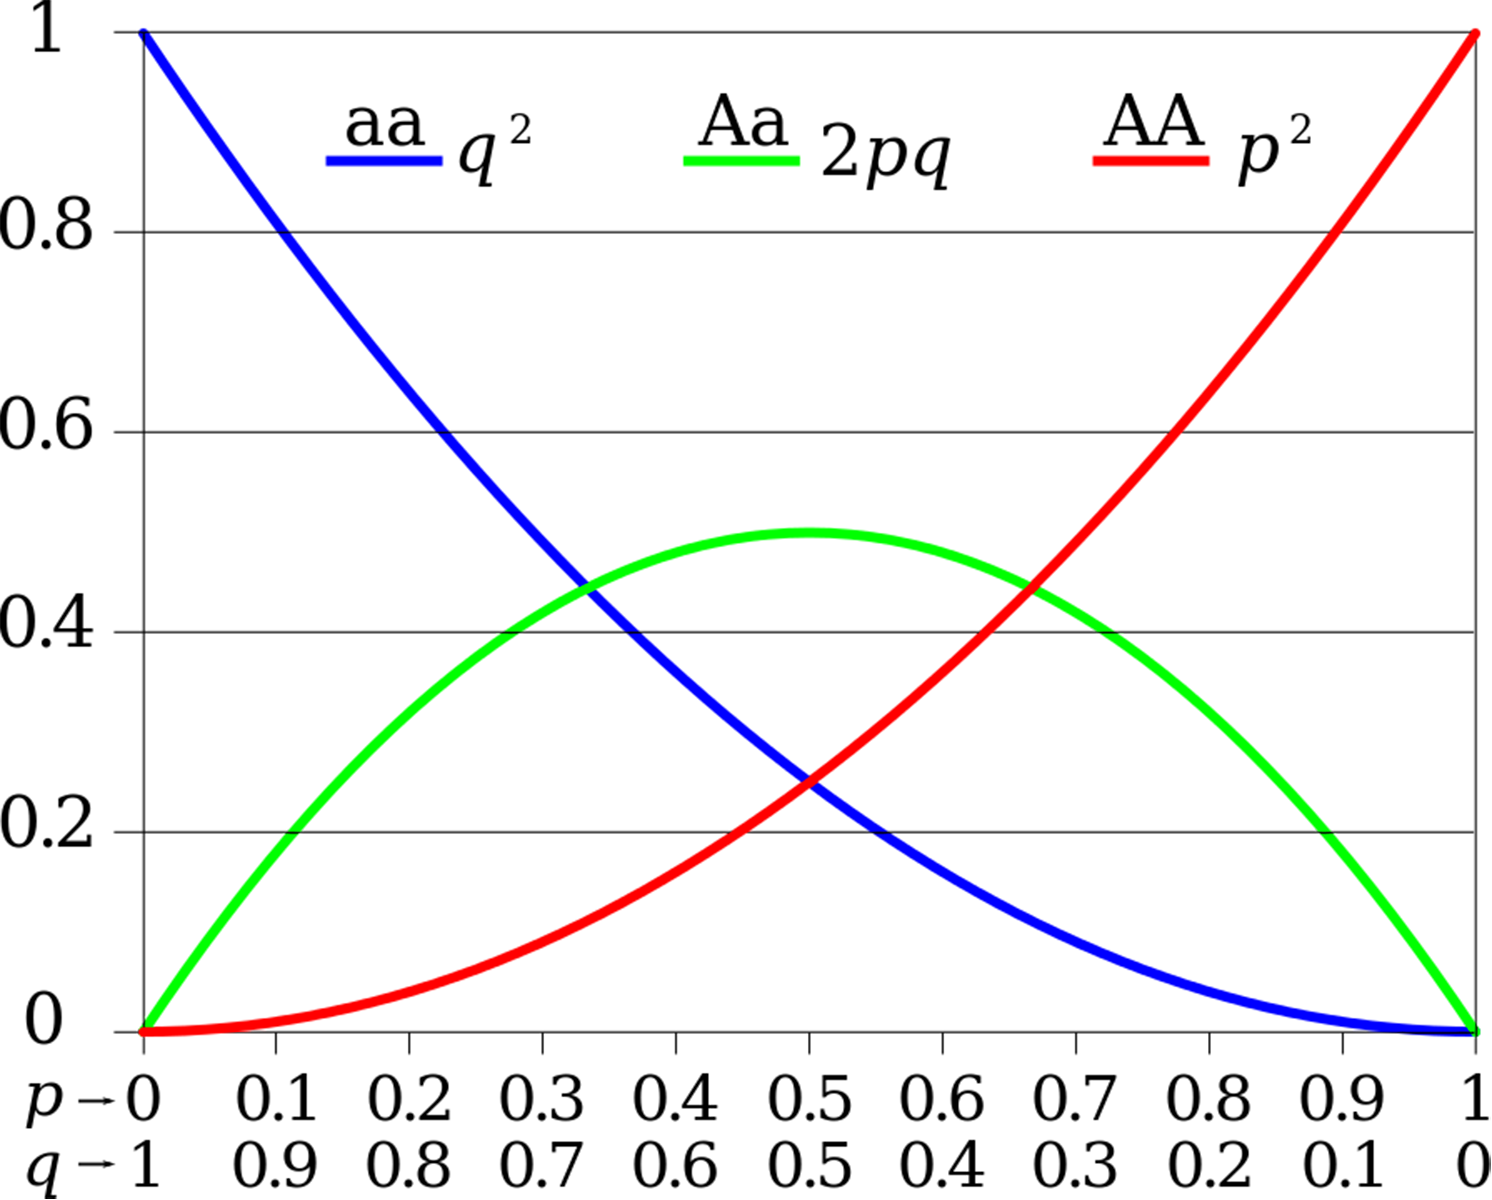
\includegraphics[width=0.4\textwidth]{images/img_7_1.png}
\caption[Αναπαράσταση ισορροπίας Hardy-Weinberg]{Αναμενόμενες συχνότητες της ισορροπίας Hardy-Weinberg για έναν γενετικό τόπο με δύο αλληλόμορφα (\href {https://commons.wikimedia.org/wiki/File:Hardy-Weinberg.svg\#/media/File:Hardy-Weinberg.svg}{πηγή: "Hardy-Weinberg" από Wikimedia Commons}).}
\label{figure:img_7_1}
\end{figure}

Ένα παράδειγμα τοποθέτησης εικόνων δίπλα-δίπλα με ενιαία λεζάντα από κάτω (εικόνα \ref{fig:double}):
\begin{figure}
\renewcommand{\figurename}{Εικόνα}
\centering
\begin{subfigure}{.5\textwidth}
  \centering
  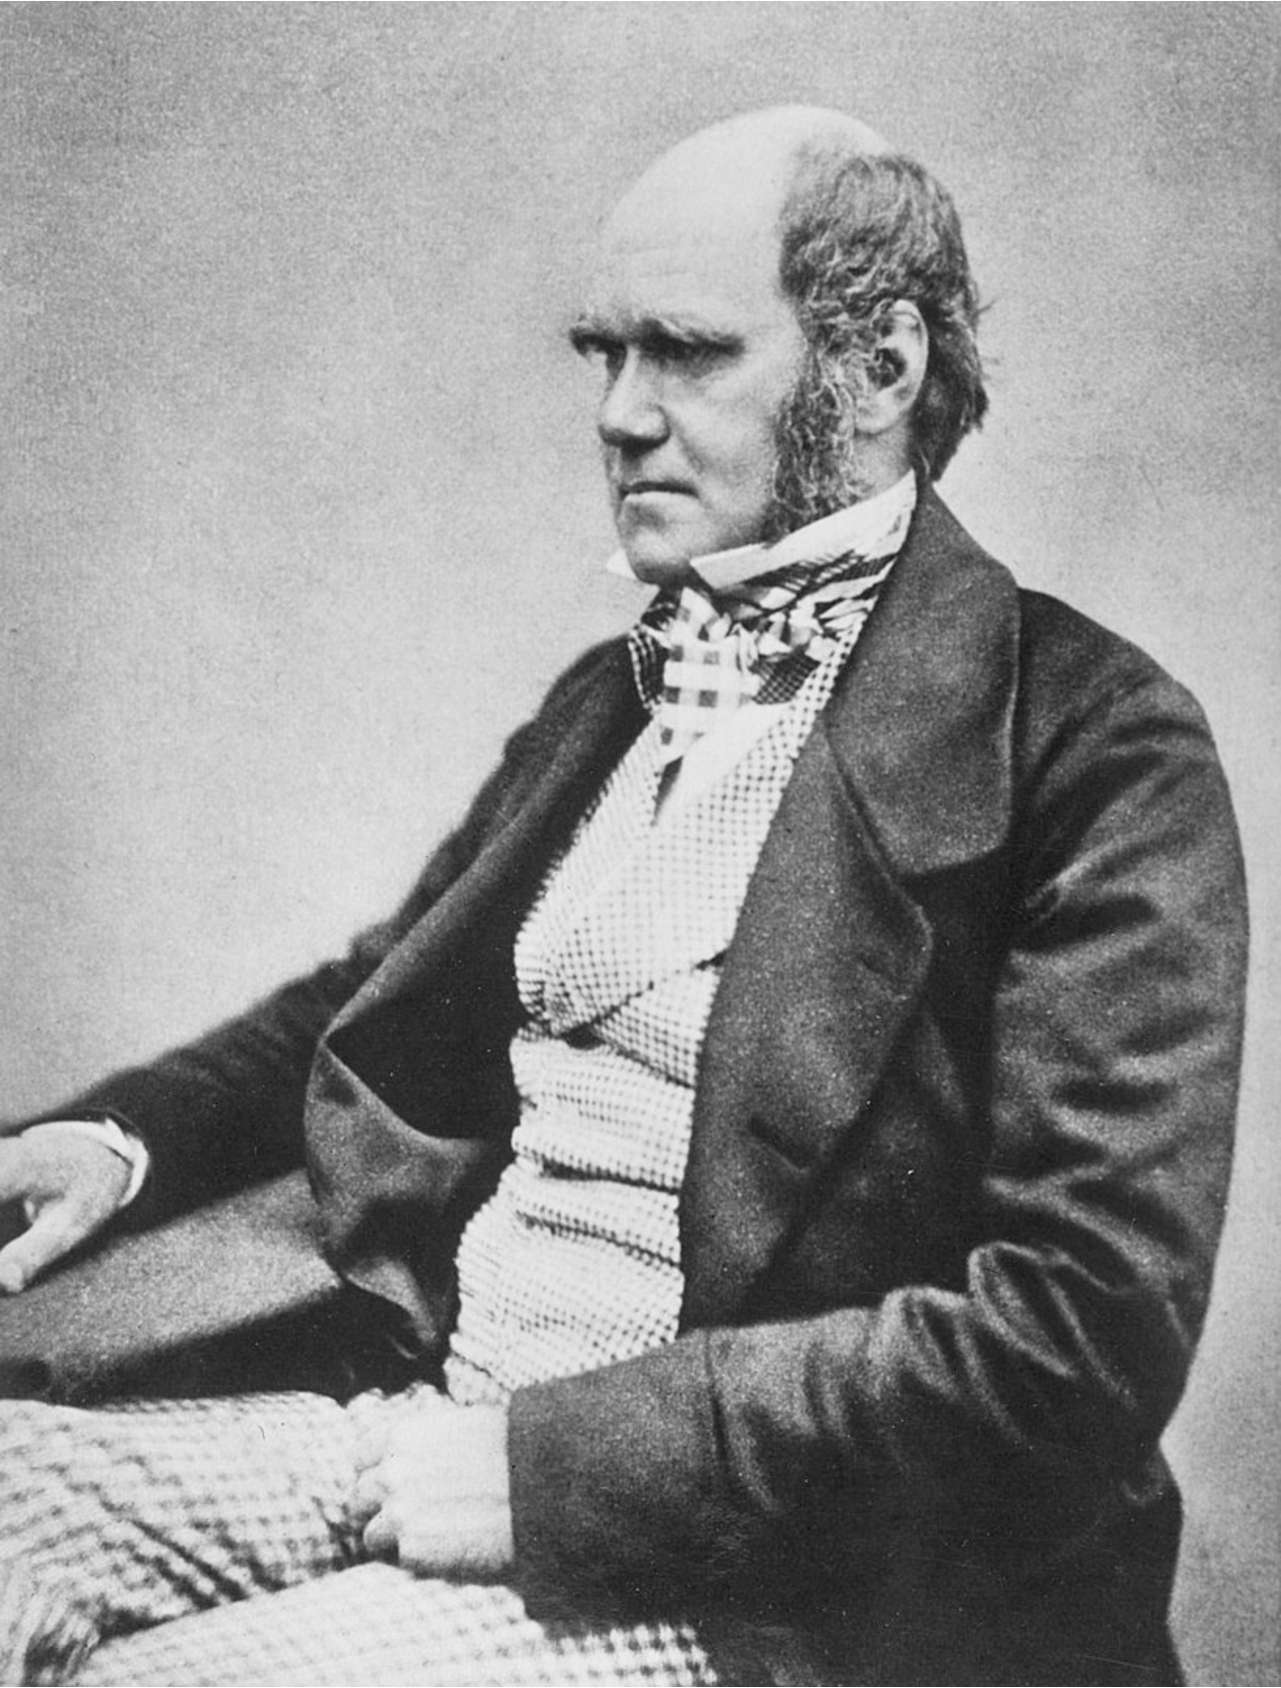
\includegraphics[width=.7\linewidth]{images/darwin.pdf}
  \caption{Charles Robert Darwin (1809-1882)}
  \label{fig:sub1}
\end{subfigure}%
\begin{subfigure}{.5\textwidth}
  \centering
  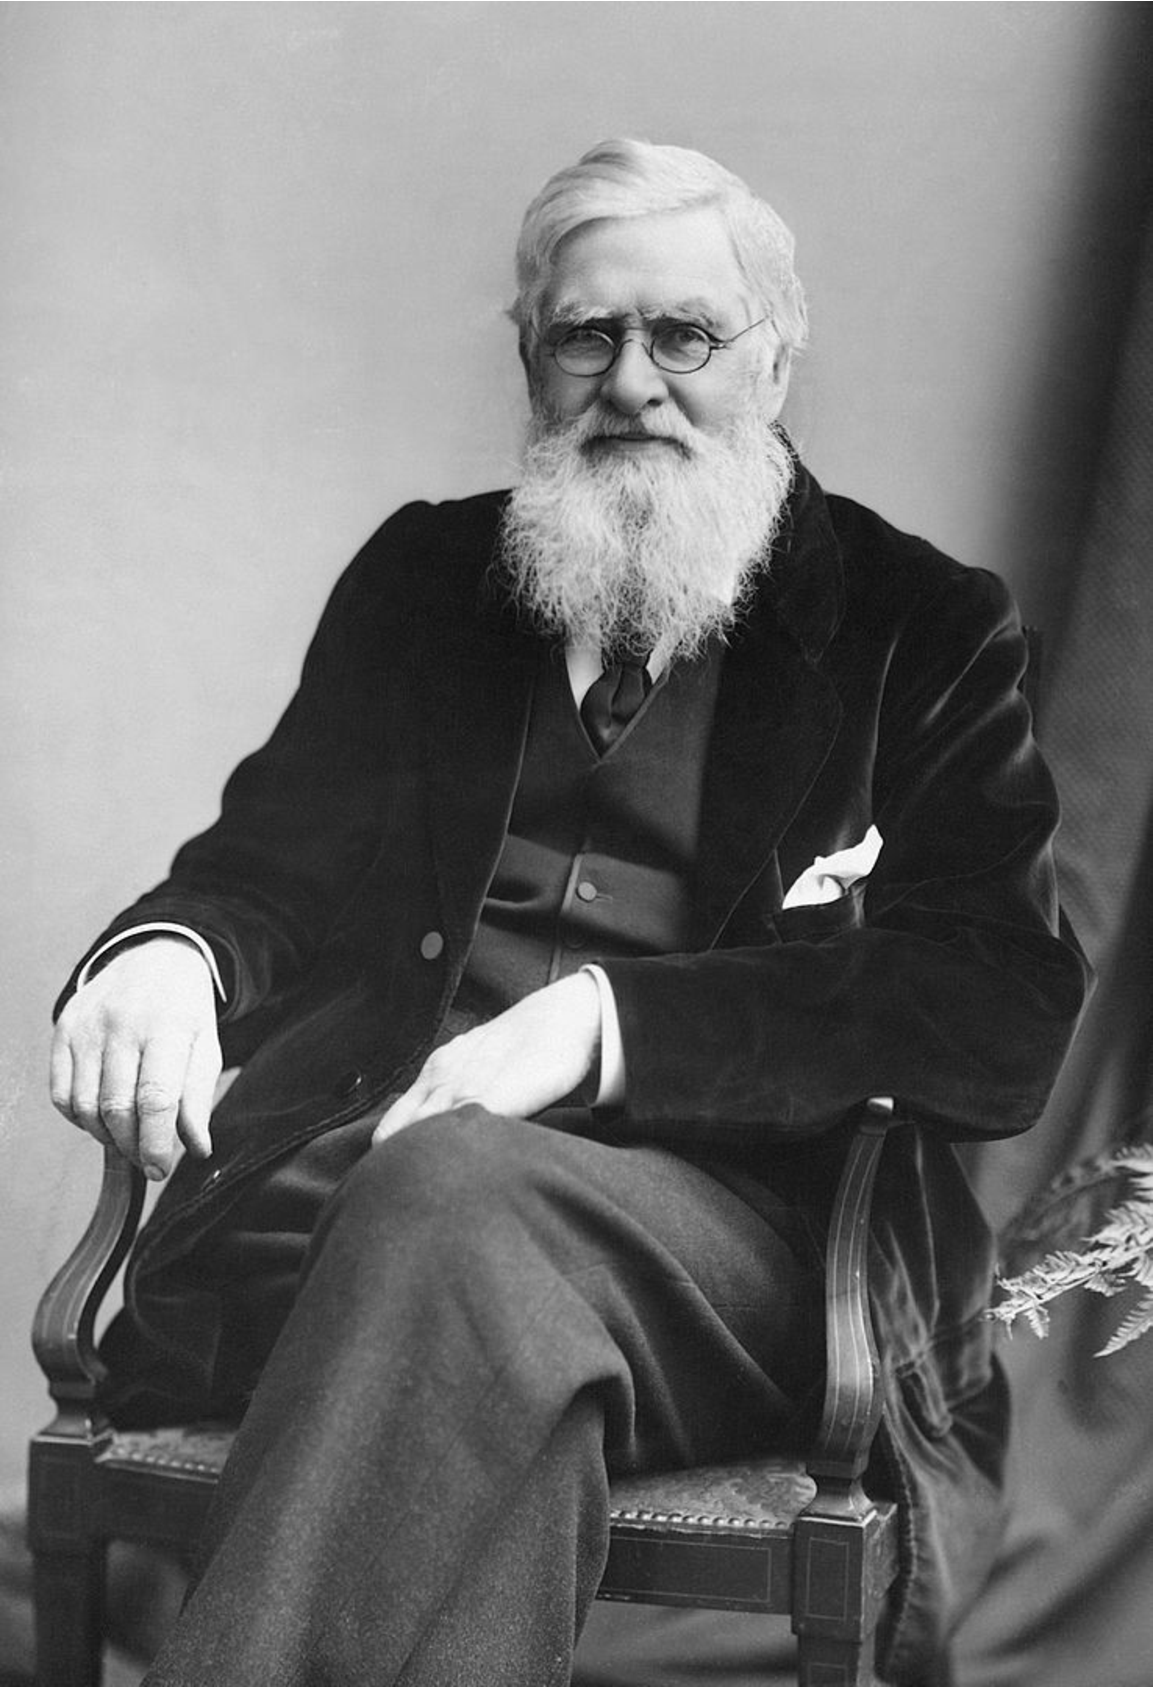
\includegraphics[width=.63\linewidth]{images/wallace.pdf}
  \caption{Alfred Russel Wallace (1823-1913)}
  \label{fig:sub2}
\end{subfigure}
\caption[Οι θεμελιωτές της εξελικτικής θεωρίας]{Οι θεμελιωτές της εξελικτικής θεωρίας. Πηγή: (α) Messrs. Maull and Fox, 1854 \href{https://commons.wikimedia.org/wiki/File:Charles_Darwin_seated_crop.jpg}{(Wikimedia Commons)}   (β) London Stereoscopic and Photographic Company, \href{https://commons.wikimedia.org/w/index.php?curid=27755581}{(Wikimedia Commons)}. }
\label{fig:double}
\end{figure}
Στην εικόνα \ref{fig:double} έχουν χρησιμοποιηθεί τα πακέτα:
\begin{verbatim}
\usepackage{caption}
\usepackage{subcaption}
\end{verbatim}
\subsection{Μαθηματικά}
\paragraph{Χρήση του περιβάλλοντος \texttt{equation}}:\\
Έχουμε τη δυνατότητα να αριθμήσουμε τις εξισώσεις μας και στη συνέχεια να αναφερθούμε σε αυτές
μέσα στο κείμενο. Παράδειγμα:\\
Το στατιστικό $X^{2}$ ισούται με:
\begin{equation}
\label{eq:7_8}
X^{2}=\sum_{i=1}^{n}\frac{(O-E)^{2}}{E}\sim^{H_{0}} X^{2}_{\mbox{1 βαθμό ελευθερίας}},
\end{equation}
όπου $O$ είναι ο παρατηρούμενος αριθμός ατόμων και $E$ ο αναμενόμενος για κάθε γονότυπο.
\paragraph{Μαθηματικά μέσα στο κείμενο}:
\begin{itemize}
\item ... είτε η υπολογισμένη τιμή του στατιστικού $X^{2}$ (βλέπε εξίσωση \ref{eq:7_8}) να υπερβαίνει την κριτική τιμή του πίνακα για ένα δοσμένο ε.$\sigma$ και ένα β.ε., δηλαδή $X^{2}> X^{2}_{1,\alpha}$ (όπως γίνεται κατανοητό η θεωρητική μας κατανομή στην περίπτωση αυτή δεν αποτελεί καλή προσαρμογή για τα δεδομένα μας),\newline
\item είτε η τιμή $p_{value}$ του ελέγχου να είναι μικρότερη από το δοσμένο επίπεδο σημαντικότητας $\alpha$, δηλαδή $p_{value} < \alpha$.
\end{itemize}

Συνεχίζοντας το παράδειγμά μας στα δεδομένα του πίνακα (\ref{table:table}) μπορούμε να υπολογίσουμε το στατιστικό $X^{2}$ και να διεξαγάγουμε τον έλεγχο καλής προσαρμογής. Η σχέση (\ref{eq:7_8}) γίνεται:

$$X^{2}= \sum_{i=1}^{n}\frac{(O-E)^{2}}{E}=\frac{(259-250.67)^{2}}{250.67}+ \frac{(495-511.45)^{2}}{511.45}+\frac{(269-260.90)^{2}}{260.90}$$
Κάνοντας τους υπολογισμούς βρίσκουμε ότι:
$$ X^{2}=1.07 $$

\subsection{Πίνακες}
Διατηρήστε τους πίνακες λιτούς για μην κουράζουν τον αναγνώστη. Ένα παράδειγμα πίνακα φαίνεται παρακάτω
(πίνακας \ref{table:table}):
\begin{table} [h] \centering \small
\caption[Συχνότητες γονότυπων του πολυμορφισμού \textit{rs1726866}]{Συχνότητες γονότυπων του πολυμορφισμού \textit{rs1726866} από επιλεγμένους πληθυσμούς του 1000 Genomes. Στο τέλος παρατίθενται οι συχνότητες από δείγμα ελληνικού πληθυσμού.}
\vspace{2mm}
\begin{tabular} {l c c c p{2cm} p{2cm} p{2.5cm}}
 \hline
 	&	&	&	&	&	&	\\
Πληθυσμός&CC	&TC	&TT	&Συχνότητα Τ ($\hat{p}$) & Συχνότητα C ($\hat{q}$) & Αναμενόμενοι ετεροζυγώτες ($E_{TC}$)\\
 \hline
	&	&	&	&	&	&	\\
CHB	&49	&41	&13	&	&	&	\\
JPT	&36	&46	&22	&	&	&	\\
TSI	&34	&51	&22	&	&	&	\\
CEU	&18	&49	&32	&	&	&	\\
GBR	&17	&43	&31	&0,58	&0,42	&45,42	\\
	&	&	&	&	&	&	\\
\hline
	&	&	&	&	&	&	\\
Σύνολο	&154	&230	&120	&	&	&	\\
	&	&	&	&	&	&	\\
\hline
	&	&	&	&	&	&	\\
Έλληνες	&269	&495	&259	&	&	&	\\
	&	&	&	&	&	&	\\
 \hline
\end{tabular}
\label{table:table}
\end{table}
\subsection{Πλαίσιο με χρωματιστό φόντο}
Παρακάτω παρουσιάζεται ένα χρωματιστό πλαίσιο με επικεφαλίδα. Πριν επιλέξετε οποιοδήποτε χρώμα σκεφτείτε
ότι πολλοί αναγνώστες θα τυπώνουν ασπρόμαυρα το κεφάλαιό σας.
\begin{kalbox}[frametitle=Περονιαία μυϊκή ατροφία]
Η περονιαία μυϊκή ατροφία ή Nόσος των Charcot-Marie-Tooth είναι μια πολυνευροπάθεια με βραδεία εξέλιξη που αρχίζει συνήθως από τους μυς που νευρώνονται από τα περονιαία νεύρα. Πρόκειται για τη συχνότερη κληρονομούμενη νευρολογική διαταραχή με συχνότητα 1/2500 στις ΗΠΑ. Διακρίνονται πολλοί τύποι της νόσου που οφείλονται σε μεταλλάξεις διαφορετικών πρωτεϊνών που σχετίζονται με τη μυελίνη. Ο τύπος 1Α προκαλείται από έναν διπλασιασμό στο χρωμόσωμα 17 που περιέχει το γονίδιο που κωδικεύει την \emph{περιφερική πρωτεΐνη της μυελίνης 22} (Peripheral Myelin Protein-22, PMP-22). Η υπερέκφρασή του προκαλεί τμηματική απομυελίνωση με συσσώρευση κυττάρων Schwann και ινών κολλαγόνου. Τα συμπτώματα αρχίζουν συνήθως στην παιδική ηλικία με χαρακτηριστική πτώση των ποδιών, καλπαστικό βάδισμα και ατροφία των μυών κάτω από τα γόνατα που μοιάζουν με πόδια πελαργού. Η νόσος δεν θεραπεύεται, αλλά έχει γενικά βραδεία εξέλιξη. Οι ασθενείς χρησιμοποιούν διάφορα βοηθήματα και αντιμετωπίζονται με φυσικοθεραπεία, εργοθεραπεία και άσκηση \cite{papan2}.
\end{kalbox}

Ο κώδικας για την παραγωγή του πλαισίου δεν είναι ενσωματωμένος στον τύπο εγγράφου \texttt{kalliposstd},
αλλά οι ενδιαφερόμενοι συγγραφείς μπορούν να τον βρουν στο βασικό αρχείο του παρόντος οδηγού.
%-------------ΑΣΚΗΣΕΙΣ - ΕΡΓΑΣΙΕΣ -----------

\section{Ασκήσεις-Εργασίες}
\newanswer{solutionsI}  % Εδώ ορίζω το είδος των απαντήσεων: solution, solutions, answers κ.λπ. Το αντίστοιχο
                      % περιβάλλον οριζεται αυτόματα και τη λύση τη γραφουμε σημειώνοντας κώδικα LaTeX.
%-------------Ασκήσεις ---------------------
\begin{exercises}[Ασκήσεις]
%---------1η άσκηση-------------
\item Η κυστική ίνωση είναι μια υπολειπόμενη πάθηση που εμφανίζεται σε 1:2.500 γεννήσεις στους Καυκάσιους. Υπολογίστε:
\begin{itemize}
\item τη συχνότητα του υπολειπόμενου παθολογικού αλληλόμορφου στον πληθυσμό,
\item τη συχνότητα του επικρατούς (φυσιολογικού) αλληλόμορφου,
\item το ποσοστό των φορέων στον πληθυσμό.
\end{itemize}
\begin{writesolutionsI} Για να απαντήσουμε το ερώτημα θεωρούμε ότι ο πληθυσμός βρίσκεται σε ισορροπία Hardy-Weinberg. Κλειδί για την απάντηση στο ερώτημα είναι η συχνότητα των ομόζυγων πασχόντων από την κυστική ίνωση ($q^2=1/2500$).
\end{writesolutionsI}
%-----------2η άσκηση -----
\item Σε ένα δείγμα φοιτητών του πανεπιστημίου έγινε δοκιμασία γεύσης του φαινυλκαρβαμιδίου (PTC). 65\% των φοιτητών ήσαν σε θέση να αντιληφθούν την πικρή γεύση. Δεδομένου ότι η δυνατότητα αντίληψης του πικρού στο φαινυλκαρβαμίδιο κληρονομείται με τον αυτοσωμικό επικρατούντα χαρακτήρα (αλληλόμορφο T), υπολογίστε τη συχνότητα των δύο αλληλόμορφων (Τ και t) στον πληθυσμό. Ποια είναι η συχνότητα του ετερόζυγου γονότυπου;
\begin{writesolutionsI}
Όπως και στην προηγούμενη περίπτωση, θα χρειαστεί να θεωρήσουμε ότι ο πληθυσμός ακολουθεί την ισορροπία Hardy-Weinberg. Στην περίπτωση αυτή γνωρίζουμε ότι το 35\% των φοιτητών είναι ομόζυγοι για το υπολειπόμενο αλληλόμορφο που συνδέεται με την αδυναμία αντίληψης του πικρού κατά τη δοκιμή του φαινυλκαρβαμιδίου (PTC).
\end{writesolutionsI}
%-----------3η άσκηση-------------
\item Ένα στα 10.000 παιδιά γεννιέται με φαινυλκετονουρία (PKU), μια μεταβολική πάθηση που χαρακτηρίζεται από νοητική καθυστέρηση. Η φαινυλκετονουρία κληρονομείται με τον σωματικό υπολειπόμενο χαρακτήρα. Ποια είναι η συχνότητα του παθολογικού αλληλόμορφου στον πληθυσμό και ποιο είναι το ποσοστό του πληθυσμού που είναι ετεροζυγώτες;
\begin{writesolutionsI}
Ακολουθήστε την ίδια μεθοδολογία με την άσκηση 1.
\end{writesolutionsI}
%-----------4η άσκηση-------------
\item H αιμορροφιλία Α είναι μια Χ-φυλοσύνδετη διαταραχή που παρουσιάζεται σε 1:5.000 γεννήσεις αρρένων. Ποια είναι η συχνότητα του παθολογικού αλληλόμορφου στον πληθυσμό; Πόσο συχνή αναμένεται να είναι η πάθηση στον γυναικείο πληθυσμό;
\begin{writesolutionsI}
Όπως και στις προηγούμενες περιπτώσεις θεωρούμε ότι ο πληθυσμός ακολουθεί την ισορροπία Hardy-Weinberg. Κλειδί για την απάντηση της ερώτησης είναι ότι η πάθηση είναι Χ-φυλοσύνδετη, άρα η συχνότητα εμφάνισης της νόσου στους άρρενες είναι η ίδια με τη συχνότητα του αλληλόμορφου που προκαλεί την αιμορροφιλία Α.
\end{writesolutionsI}
%-----------5η άσκηση-------------
\item Σε έναν διαλληλικό γενετικό τόπο ποια συχνότητα αλληλόμορφων θα εμφανίζει διπλάσιο αριθμό υπολειπόμενων ομοζυγωτών σε σχέση με τους ετεροζυγώτες;
\begin{writesolutionsI} Στην περίπτωση αυτή οι ομοζυγώτες είναι διπλάσιοι από τους ετεροζυγώτες. Άρα ισχύει: $$2\times q^2=2pq$$.
\end{writesolutionsI}
\end{exercises}
\closesolutionsI
%----------Τέλος των ασκήσεων ----------

%------------ΕΡΓΑΣΙΕΣ ------------------
\newanswer{solutionsII}
\begin{exercises}[Εργασίες]
%------------1η εργασία ------------------
\item Επισκεφθείτε τον περιηγητή  \href{http://www.ensembl.org}{ENSEMBL} και αναζητήστε δεδομένα για τους μονονουκλεοτιδικούς πολυμορφισμούς \textit{rs4988235} και \textit{rs182549}, που σχετίζονται με την παρατεινόμενη έκφραση της λακτάσης. Επιλέξτε το εικονίδιο \textit{Population Genetics} και κατεβάστε με τη μορφή αρχείου φύλλου εργασίας τα δεδομένα του πίνακα με τις συχνότητες των γονότυπων από το 1000 Genomes. Επιλέξτε τα δεδομένα από τους ακόλουθους πληθυσμούς: GBR, TSI, ΥRI, MAG, MXL, PEL, CHB, JPT, PJL, STU, καθώς και τα συγκεντρωτικά στοιχεία για AFR, AMR, EUR, EAS, SAS.
\begin{itemize}
\item Πραγματοποιήστε έλεγχο των δεδομένων για την ισορροπία Hardy-Weinberg με την εφαρμογή De Finetti Generator.
\item Απεικονίστε στον χάρτη που θα βρείτε στη διεύθυνση \url{https://commons.wikimedia.org/wiki/File:World_map_between_2003_and_2005.png#filelinks} τις συχνότητες των αλληλόμορφων ανά ήπειρο και πληθυσμό.
\item Γράψτε μια μικρή παράγραφο με τις παρατηρήσεις και τα συμπεράσματα που βγάλατε από την εργασία σας.
\end{itemize}
\begin{writesolutionsII}
Συγκρίνετε τα αποτελέσματα της έρευνάς σας στους διάφορους πληθυσμούς. Συμβουλευτείτε την ακόλουθη βιβλιογραφία, ανατρέχοντας στη βιβλιοθήκη:
<<Γαλακτοφιλία και γαλακτοφοβία>> στο Harris M., \textit{Η ιερή αγελάδα και ο βδελυρός χοίρος. Προβλήματα διατροφής και πολιτισμού}, Τροχαλία, Αθήνα, 1987.
\end{writesolutionsII}
%------------2η εργασία ------------------
\item Εξετάζοντας τη βιβλιογραφία στο τέλος του κεφαλαίου και τις διαδικτυακές πηγές του  \href{http://omim.org}{OMIM} και του \href{http://www.ncbi.nlm.nih.gov/books/NBK1116/}{Gene Reviews} απαντήστε στα παρακάτω ερωτήματα:
\begin {itemize}
\item Ποιες παθήσεις συνδέονται με το γονίδιο PRNP;
\item Τι είναι τα prions;
\item Τι είναι η νόσος Kuru;
\item Ποιο είναι το κοινωνικό και ανθρωπολογικό πλαίσιο των ιδιόρρυθμων διαιτητικών συνηθειών των Φόρε που προσβάλλονταν από τη νόσο Kuru;
\end{itemize}
\begin{writesolutionsII}
Βοηθητικά μπορείτε να ανατρέξετε στις παρακάτω βιβλιογραφικές αναφορές:
α) Harris M., \textit{Η ιερή αγελάδα και ο βδελυρός χοίρος. Προβλήματα διατροφής και πολιτισμού}, Τροχαλία, Αθήνα, 1987.
β) Brown M. J., \textit{Explaining Culture Scientifically}, University of Washington Press, Seattle, 2008.
γ) Lindenbaum S., «Understanding Kuru: The Contribution of Anthropology and Medicine»,\textit{Phi\-lo\-so\-phi\-cal Transactions of the Royal Society B: Biological Sciences}, 2008, 363(1510): 3715-3720.
δ) Mead S, Whitfield J, Poulter M. et al., <<Genetic Susceptibility, Evolution and the Kuru Epidemic>>. \textit{Philosophical Transactions of the Royal Society B: Biological Sciences}, 2008, 363(1510): 3741-3746.
\end{writesolutionsII}
\end{exercises}
\closesolutionsII
%----------------- Εδώ τελειώνουν οι ασκήσεις - εργασίες και οι απαντήσεις τους ------

%-----------------Βιβλιογραφία -------------------
\printbibliography[heading=biboption]
\end{refsection}


%-------------------------------------------------------------
%			ΠΑΡΑΡΤΗΜΑΤΑ
%-------------------------------------------------------------

\part{Παραρτήματα}
\appendix
\begin{refsection}
\chapter{Πίνακες}
\section{Σύμβολα νουκλεοτιδίων}\label{noukl_symbols}
\begin{table}[ht] \centering \small
\caption[Πίνακας συμβόλων νουκλεοτιδίων]{Πίνακας συμβόλων που χρησιμοποιούνται στα αρχεία που περιέχουν νουκλεοτιδικές αλληλουχίες.}
\vspace{2mm}
\begin{tabular} {c l}
 \hline
	&	\\
\textbf{Σύμβολο νουκλεοτιδίου}	& \textbf{Επεξήγηση} \\
	&	\\
 \hline
A 	& 	A\\
C	& 	C\\
G 	& 	G \\
T	& 	T \\
U	& 	U\\
R 	& 	A ή G\\
Y & 		C, T ή U\\
K	&	G, T ή U\\
M	&	A ή C\\
S	&	C ή G\\
W	&	A, T ή U\\
B	&	Όχι A (δηλαδή C, G, T ή U)\\
D	&	Όχι C (δηλαδή A, G, T ή U)\\
H	&	Όχι G (δηλαδή A, C, T ή U)\\
V	&	Ούτε T ούτε U (δηλαδή A, C ή G)\\
N	&	A, C, G, T, U\\
X	&	Μεταμφιεσμένο\\
-	&	Χάσμα ασαφούς μήκους\\
\hline
\end{tabular}
\label{table:table_2_2}
\end{table}
\newpage
\section{Σύμβολα αμινοξέων}\label{aminoacid_symbols}
\begin{table}[ht] \centering \small
\caption[Πίνακας συμβόλων αμινοξέων]{Πίνακας συμβόλων που χρησιμοποιούνται στα αρχεία που περιέχουν αλληλουχίες αμινοξέων (πρωτεΐνες).}
\vspace{2mm}
\begin{tabular}  {c c l  p{6cm}}
 \hline
	&	&&\\
\textbf{Σύμβολο}	&\textbf{Συντομογραφία}	&\textbf{Ονομασία}&\textbf{Κωδικόνια}\\
	&	&&\\
\hline
	&	&&\\
A	&Ala	&Aλανίνη&GCT, GCC, GCA, GCG\\
B	&Asp ή Asn	&Aσπαρτικό οξύ (D) ή Aσπαραγίνη (N)& GAT, GAC - AAT, AAC\\
C	&Cys	&Κυστεΐνη&TGT, TGC\\
D	&Asp	&Aσπαρτικό οξύ&GAT, GAC\\
E	&Glu	&Γλουταμικό οξύ&GAA, GAG\\
F	&Phe	&Φαινυλαλανίνη&TTT, TTC\\
G	&Gly	&Γλυκίνη&GGT, GGC, GGA, GGG\\
H	&His	&Ιστιδίνη&CAT, CAC\\
I	&Ile	&Ισολευκίνη&ATT, ATC, ATA\\
J	&Leu ή Ile	&Λευκίνη (L) ή Iσολευκίνη (I)&TTA, TTG, CTT, CTC, CTA,CTG - ATT, ATC, ATA\\
K	&Lys	&Λυσίνη&AAA, AAG\\
L	&Leu	&Λευκίνη&TTA, TTG, CTT, CTC, CTA,CTG\\
M	&Met	&Mεθειονίνη&ATG\\
N	&Asn	&Aσπαραγίνη&AAT, AAC\\
O	&Pyl	&Πυρολυσίνη&\\
P	&Pro	&Προλίνη&CCT, CCC, CCA, CCG\\
Q	&Gln	&Γλουταμίνη&GGT, GGC, GGA, GGG\\
R	&Arg	&Aργινίνη&CGT, CGC, CGA, CGG, AGA, AGG\\
S	&Ser	&Σερίνη&TCT, TCC, TCA, TCG, AGT, AGC\\
T	&Thr	&Θρεονίνη&ACT, ACC, ACA, ACG\\
U	&Sec	&Σεληνοκυστεΐνη&\\
V	&Val	&Βαλίνη&GTT, GTC, GTA, GTG\\
W	&Trp	&Tρυπτοφάνη&TGG\\
Y	&Tyr	&Tυροσίνη&TAT, TAC\\
Z	&Glu ή Gln	&Γλουταμικό οξύ (E) ή Γλουταμίνη (Q)&GAA, GAG - CAA, CAG\\
X	&	&Οποιοδήποτε αμινοξύ&\\
*	&STOP	&Τερματισμός μετάφρασης&TAA, TGA, TAG\\
-	&	&Χάσμα ασαφούς μήκους&\\
	&	&&\\
\hline
\end{tabular}
\label{table:table_2_3}
\end{table} 
\end{refsection}

\chapter{Απαντήσεις ερωτήσεων - Λύσεις ασκήσεων}
\begin{refsection}
\section{Κεφάλαιο 7}\label{sol_CH-7}
\subsection{Λύσεις ασκήσεων}
\inputsolutionsI
\subsection{Εργασίες}
\inputsolutionsII
\end{refsection}


%------- Οπισθόφυλλο  ----------------------------------------

\includepdf[pages=3-4]{images/KOY_cover.pdf}
\end{document}
